\chapter{Exploratory data analysis of LPs using t-SNE} 

\label{chapter5} 

\section{Introduction}

LPs can be used to understand the consumption patterns of appliances or buildings.
The one thing they do not offer is a comparison between activation patterns.
To achieve this we can utilize various dimensionality reduction algorithms. 
In the process of dimensionality reduction, these algorithms map similar LPs closer together compared to dissimilar LPs.
This enables us to have an insight into similar activation patterns across various entities.
It enables us to visualize and compare LPs of buildings and appliances, to find the differences and similarities in their activation patterns.

In this chapter, we will explore the use of t-distributed stochastic neighbor embedding (t-SNE) for Exploratory Data Analysis (EDA) on LPs.
The t-SNE is a non-linear dimensionality reduction algorithm, used to visualize high dimensional data in usually two or three dimensions.
We will delve into the details of what t-SNE is and how can it be applied to the LPs.

To achieve this goal, we will first provide a brief overview of t-SNE and its application to LPs.
Next, we will describe our methodology for using t-SNE to analyze LPs and compare activation patterns.
Finally, we will present the results of our analysis and discuss their implications for understanding energy consumption patterns.

The clustering of similar LPs was researched many times before, as it was described in related work Chapter \ref{chapter2}.
We will be working with dimensionality reduction, where clusters are usually formed as a side product.
The following clustering publications are worth mentioning.
We have seen that authors \cite{GERBEC2005}, \cite{Jeong2021} and \cite{Joana2012} have clustered regular one-dimensional LPs, as well as with 2D image-based load profiling in publications published by authors \cite{Park2019}. 

The publication by authors \cite{sne_energ} compared various dimensionality reduction techniques for clustering and visualization of LPs.
Their goal was to compare Principal Component Analysis, Isometric Feature Mapping, Sammon Mapping, Locally Linear Embedding and Stochastic Neighbor Embedding.
They used daily power LPs from residential and industrial areas.
This publication was of the closest resemblance to our goals, that we were able to find. 

In all cases, work has been done with the power LP, whereas in this case, we will try to find similarities between activation profiles using a t-SNE algorithm.
Most of the publications used single-time dimensions, whereas we will use two-time dimensions.

Although the use-cases were presented in-depth in Chapter \ref{chapter2}, it is worth mentioning one specific use case.
The increasing price of energy resources, could lead to over-saving and living in cool homes.
By using similarity metrics between profiles across different buildings, it would be possible to detect outliers when it comes to heating. 
With this approach, it would be possible to detect users, that are living in below-average cool homes and offer them cheaper plans. 

\section{Methodology}

\subsection{LPs}

\subsubsection{Weekly-Daily LP}

During testing, a weekly-daily LP constructed from a month of data will be used.
Y-axis will present the days in a week and X-axis presents the hours in a day.
Weekdays are labeled from 0 to 6, and hours from 0 to 23.
Since we are working with images, the origin is placed in the upper-left corner. 
This means that a pixel in the upper-left corner presents the first hour of a week,
this would be a Monday from midnight to one o'clock. 
The lower-right corner presents the last hour of the week.
Since there are roughly 4 weeks in each month, each pixel will present 4 samples. 
One such example of profiles that we will use, was already presented in Chapter \ref{chapter4} with Figure \ref{fig:wm_hm_weekly}.
For practical reasons, we are presenting it again here with Figure \ref{fig:wm_hm_weekly_2}.

\begin{figure}[H]
	\centering
	\caption{Weekly per-appliance LP}
	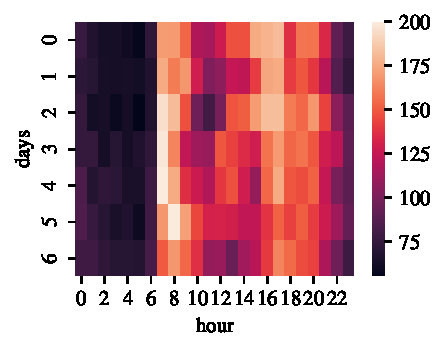
\includegraphics[]{../Figures/LPS/wm_hm_weekly.pdf}
	\label{fig:wm_hm_weekly_2}
\end{figure}


\subsubsection{Bag of Appliances LP}

Another LP that will be used at the end of this Chapter will be the bag-of-appliances LP.
The profile was presented and analyzed in depth in Chapter \ref{chapter4} and was presented in Figure \ref{fig:BOA}.
But again, for ease-of-use purposes, we will summarize the profile here.

\begin{figure}[H]
	\centering
	\caption{Universal presentation of per-building per-appliance LP}
	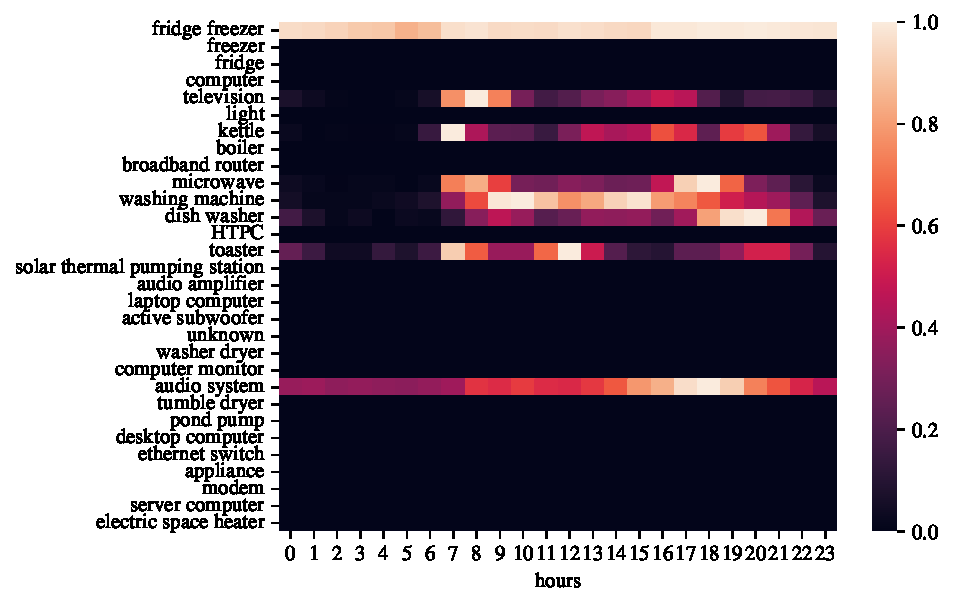
\includegraphics[width=1\textwidth]{../Figures/LPS/BOA.pdf}
	\label{fig:BOA2}
\end{figure}

To build the profile seen in Figure \ref{fig:BOA2}, we used the data from all 5 datasets and made a list of the most commonly used appliances.
Only the top 30 appliances were selected.
This enables us to have the same LP for all buildings, and thus enables us to see how the usage differs across them.
One problem that arises here is the missing appliances.
These appliances present themselves as a black line.
A lot of missing appliances may cause the image to be primarily black,
which could cause trouble for the algorithm processing this as an image.

\subsection{Normalisation}
\label{ssec:norm}
Activations portrayed in a heatmap must always be normalised in order for color (heat) to be propely mapped.
We need to ensure that the LPs fed into t-SNE match our perception in order to achieve meaningful results we can interpret.
To achieve this we will use min-max scaling seen in Equation \ref{eq:minmax} below.

\begin{equation}
	\label{eq:minmax}
	x_{norm} = \frac{x - x_{min}}{x_{max} - x_{min}}
\end{equation}
	
 Where $x$ is the value being scaled, $x_{min}$ is the minimum number of activations in the LP, $x_{max}$ is the maximum number of activations in the LP, and $x_{norm}$ is the output normalised value.
	
\subsection{Data}

We have on average roughly one year of data per building. 
In some cases few weeks and in others up to 5 years for some appliances.
By slicing this data into 1-month-long intervals and converting them to LPs we were able to obtain 5218 samples.

More detailed methodological approaches were discussed in Section \ref{ssec:data}.

\subsection{T-SNE Algorithm}

The t-SNE \cite{tsne2} or t-distribution stochastic neighboring embedding is a method for portraying high dimensional 
data in low dimensional space. This process is also known as dimensionality reduction.

One of the well-known dimensionality reduction algorithms is PCA.
The key difference between the two is that one is linear, and the other is non-linear.
PCA, linear, projects data in new space and finds the one with the least variance between data points.
SNE \cite{sne1}, non-linear, is composed of two main parts. The first one is 
converting the high-dimensional Euclidean distances between data points into conditional probabilities that represent similarities \cite{sne1}.
The pairs with high similarity have a high probability, and pairs with lower a low probability.
Second, it uses Kullback-Leibler divergence to minimize it with respect to a location on a map.
To achieve this it uses gradient descent to minimize the cost function.
Over many iterations, similar data points should be close together and far away from dissimilar objects.
Similar data points usually form clusters. 
t-SNE uses SNE as a basis, except that it uses t-student distribution instead of normal to calculate the similarity.

A good example that showcases the non-linearity of t-SNE can be seen in Figure \ref{fig:tsne_diagram}.
In this simple task, projecting all data points to the y-axis would leave us with a different solution than the one we can see on the right.
%TODO add simple projection
\begin{figure}[H]
    \centering
    \begin{tikzpicture}
        % Draw the input figure
        \node (input) at (0,0) {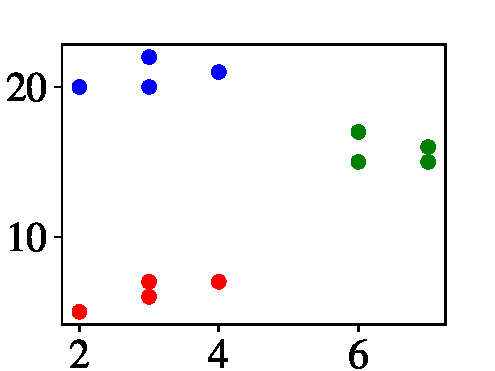
\includegraphics[width=4cm]{Figures/TSNE/DEMO/input.pdf}};
        
        % Draw the output figure
        \node (output) at (6,0) {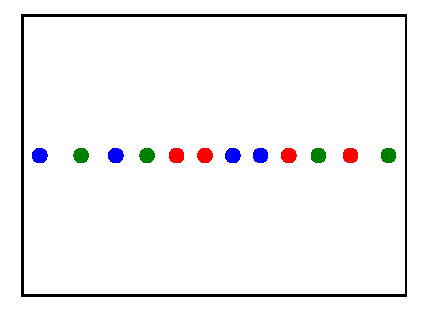
\includegraphics[width=4cm]{Figures/TSNE/DEMO/iteration_4.pdf}};
        
        % Add arrows between the figures
        \draw[->, thick] (input.east) -- (output.west) node[midway, above] {t-SNE};
    \end{tikzpicture}
    \caption{2D data point transformed into 1D data point using t-SNE}
    \label{fig:tsne_diagram}
\end{figure}

In order to calculate the t-SNE for a set of data points, we first need to calculate the conditional probability.
This is calculated based on the Equation \ref{eq:pij} below.
The author of t-SNE Van der Mateen \cite{tsne2} states:
“The similarity of datapoint $x_j$ to datapoint $x_i$ is the conditional probability, $p_{ij}$, that $x_i$ would pick $x_j$ as its neighbor if neighbors were picked in proportion to their probability density under a Gaussian centered at $x_i$.” 

\begin{equation}
\label{eq:pij}
p_{ij} = \frac{\exp(-\lVert x_i - x_j \rVert^2/2\sigma_i^2)}{\sum_{k \neq l} \exp(-\lVert x_k - x_l \rVert^2/2\sigma_i^2)} \
\end{equation}

In Equation \ref{eq:pij} $x_i$ and $x_j$ are two data points and $|x_i - x_j|$ is the Euclidean distance between the two.
The nominator in Equation \ref{eq:pij} is equal to the similarity between two points normalized by the variance $2\sigma_i^2$.
The whole expression is run through $exp()$ function to ensure the value stays positive and within boundaries.
The denominator in Equation \ref{eq:pij} serves as a normalisation factor, to ensure that the sum of probabilities for data point $x_i$ will sum to 1.

The $\sigma_i$ is also known as Gaussian bandwidth, Gaussian kernel or just variance is picked for each data point based on the number of neighbors in its vicinity.
In areas where data points are more crowded, $\sigma_i$ is usually smaller than in less crowded areas.
It is pre-calculated for every point using binary search. 
A search is complete when $\sigma_i$ outputs probability distribution $P_i$ that matches user-defined perplexity $Perp(P_i)$.

$$Perp(P_i) = 2^{H(P_i)}$$

Here, $H(P_i)$ is the entropy of the conditional probability distribution $P_i$.
The entropy of conditional probability distribution is a measure of perplexity.
Perplexity is one of the parameters defined by the user, and it's used as a measure of the number of effective neighbors, between which we will compute similarities.
High perplexity means that the distribution of the Gaussian kernel will be wide and contain more data points between which similarity will be computed.
Low perplexity means that the kernel will be narrow, so fewer data points will fit into it and therefore fewer data points will be compared.

The output of the algorithm is a map of every data point $y_i$.
These points are low dimensional counterparts of $x_i$.
Usually, these data points contain a comprehensible number of dimensions where $y_i \in \mathbb{R}^2$ or $\mathbb{R}^3$. 
Similarly, as in equation \ref{eq:pij} we can now use low dimensional data points $y_i$ and $y_j$ to calculate probability $q_{ij}$ in equation \ref{eq:gij}.
Here, t-student distribution with one degree of freedom is utilized to calculate the similarities.

\begin{equation}
\label{eq:gij}
q_{ij} = \frac{(1+\lVert y_i - y_j \rVert^2)^{-1}}{\sum_{k \neq l} (1+\lVert y_k - y_l \rVert^2)^{-1}} 
\end{equation}

$q_{ij}$ is again a conditional probability of finding $y_i$ and $y_j$ near each other but for fewer dimensions.

Setting up a cost function, which tries to minimize the difference between $q_{ij}$ and $p_{ij}$ should result in a low dimensional map where similar points should be near eachother.
The cost function is also known as Kullback-Leibler divergence seen in Equation \ref{eq:Klle}. 
The equation is the sum of all pairwise similarities between low and high-dimensional data points.
The smaller the $C$ the closer the similar data points are in low dimensional space.

\begin{equation}
\label{eq:Klle}
 C = \sum_{i \neq j}^n p_{ij} \log \frac{p_{ij}}{q_{ij}}
\end{equation}

The similarity is achieved over many iterations where we use gradient descent to minimize the Kullback-Leibler divergence seen in Equation \ref{eq:Klle}. 
The process can be seen in Figure \ref{fig:tsne_iterations_arrows}.

\begin{figure}[H]
    \centering
    \begin{tikzpicture} 
        % Draw the first subfigure
        \node (tsne1) at (0,0) {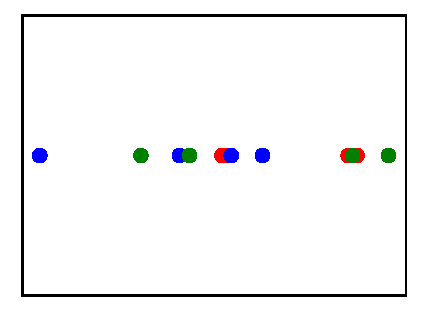
\includegraphics[width=0.25\textwidth]{Figures/TSNE/DEMO/iteration_1.pdf}};
        \node[above] at (tsne1.north) {0 iters};
        
        % Draw the second subfigure
        \node (tsne2) at (0.35\textwidth,0) {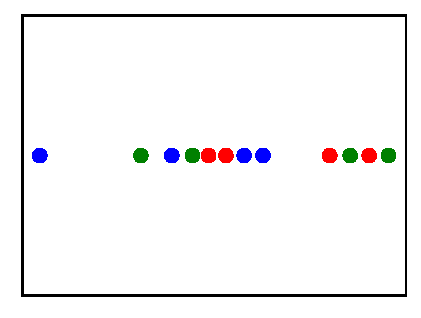
\includegraphics[width=0.25\textwidth]{Figures/TSNE/DEMO/iteration_2.pdf}};
        \node[above] at (tsne2.north) {150 iters};
        
        % Draw the third subfigure
        \node (tsne3) at (0.7\textwidth,0) {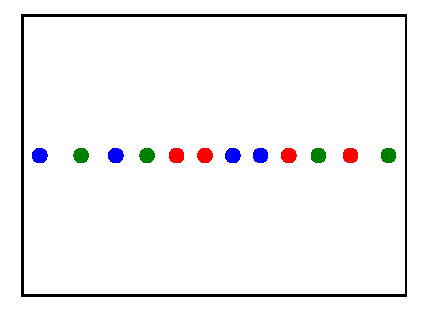
\includegraphics[width=0.25\textwidth]{Figures/TSNE/DEMO/iteration_4.pdf}};
        \node[above] at (tsne3.north) {400 iters};
        
        % Add arrows between the subfigures
        \draw[->, thick] (tsne1.east) -- (tsne2.west);
        \draw[->, thick] (tsne2.east) -- (tsne3.west);
    \end{tikzpicture}
    \caption{Iterations of t-SNE}
	\par
    \par\footnotesize{The input data can be seen in \ref{fig:tsne_diagram} }
	\label{fig:tsne_iterations_arrows}
\end{figure}


In our case, two dimensions will be used. Since this is a non-linear dimensionality reduction,
the axis usually presents dimensions that are hard to comprehend by the brain. 
It is important to keep in mind that the resulting low-dimensional representation is not necessarily interpretable in the same way as the original high-dimensional data.
This also means that the axes labels on the graphical presentations are meaningless.
In our case, we labeled the two axes as $dimension-1$ and $dimension-2$.

\section{Results}

The results will be presented in three subsections

\begin{itemize}
	\item Per-building LP
	\item Per-appliance LP
	\item Per-building per-appliance LP
\end{itemize}

%Most of the focus will be done on the per-appliance LP since it is the most universal.

The following figures are best viewed in color and a digital format. 
In the analysis, the reader can use the first figures to identify buildings and the second to identify the patterns and actual LPs.
Readers reading the digital version should have the ability to zoom into each cluster and see the actual samples. 
Readers reading a paper version can still explore the high-resolution figures online via the provided link below every figure.

\subsection{Results for Per-Building LPs}
%TODO
\label{ssec:res_pb_lp}
This LP is useful when it comes to comparing how 
activation patterns change over buildings and datasets.
Per-building data uses combined activations of all appliances to present 
the aggregated usage pattern.  

This section will first address non-normalized LPs and later move on to normalized LPs.
We have already addressed the methodology on normalization in Section \ref{ssec:norm}.
By normalizing the data we are essentially removing information from the LP.
This information contains knowledge of the number of the appliances in building and their usage intensity.
Knowing the two could be useful in scenarios where we are analyzing the magnitude of usage and not the patterns themselves.

Figure \ref{fig:tsne_scatter_non_norm_all} is using non-normalized data, meaning
the number of appliances in a building will affect the end LP.
The algorithm could pick up on how many and how much appliances are being used.
In some cases, such as energy poverty detection, this information is useful, as we are searching for buildings that exhibit reduced activation patterns.

\begin{figure}[H]
	\centering
	\caption{Projection of per-building LPs}
	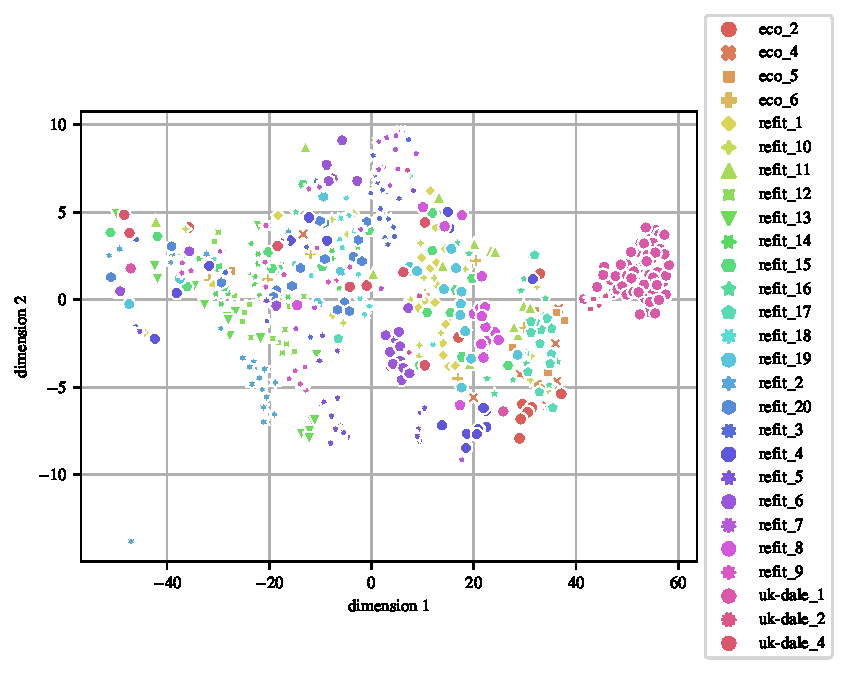
\includegraphics[]{Figures/TSNE/TSNE_per_building/scatter_per_building.pdf}
	\label{fig:tsne_scatter_non_norm_all}
	\par
	\par\footnotesize{Full resolution figure: \url{https://github.com/jenkoj/msc/tree/main/Figures/TSNE/TSNE_per_building/scatter_per_building.pdf}}
\end{figure}

\begin{figure}[H]
	\centering
	\caption{Projection of per-building LPs with actual samples}
	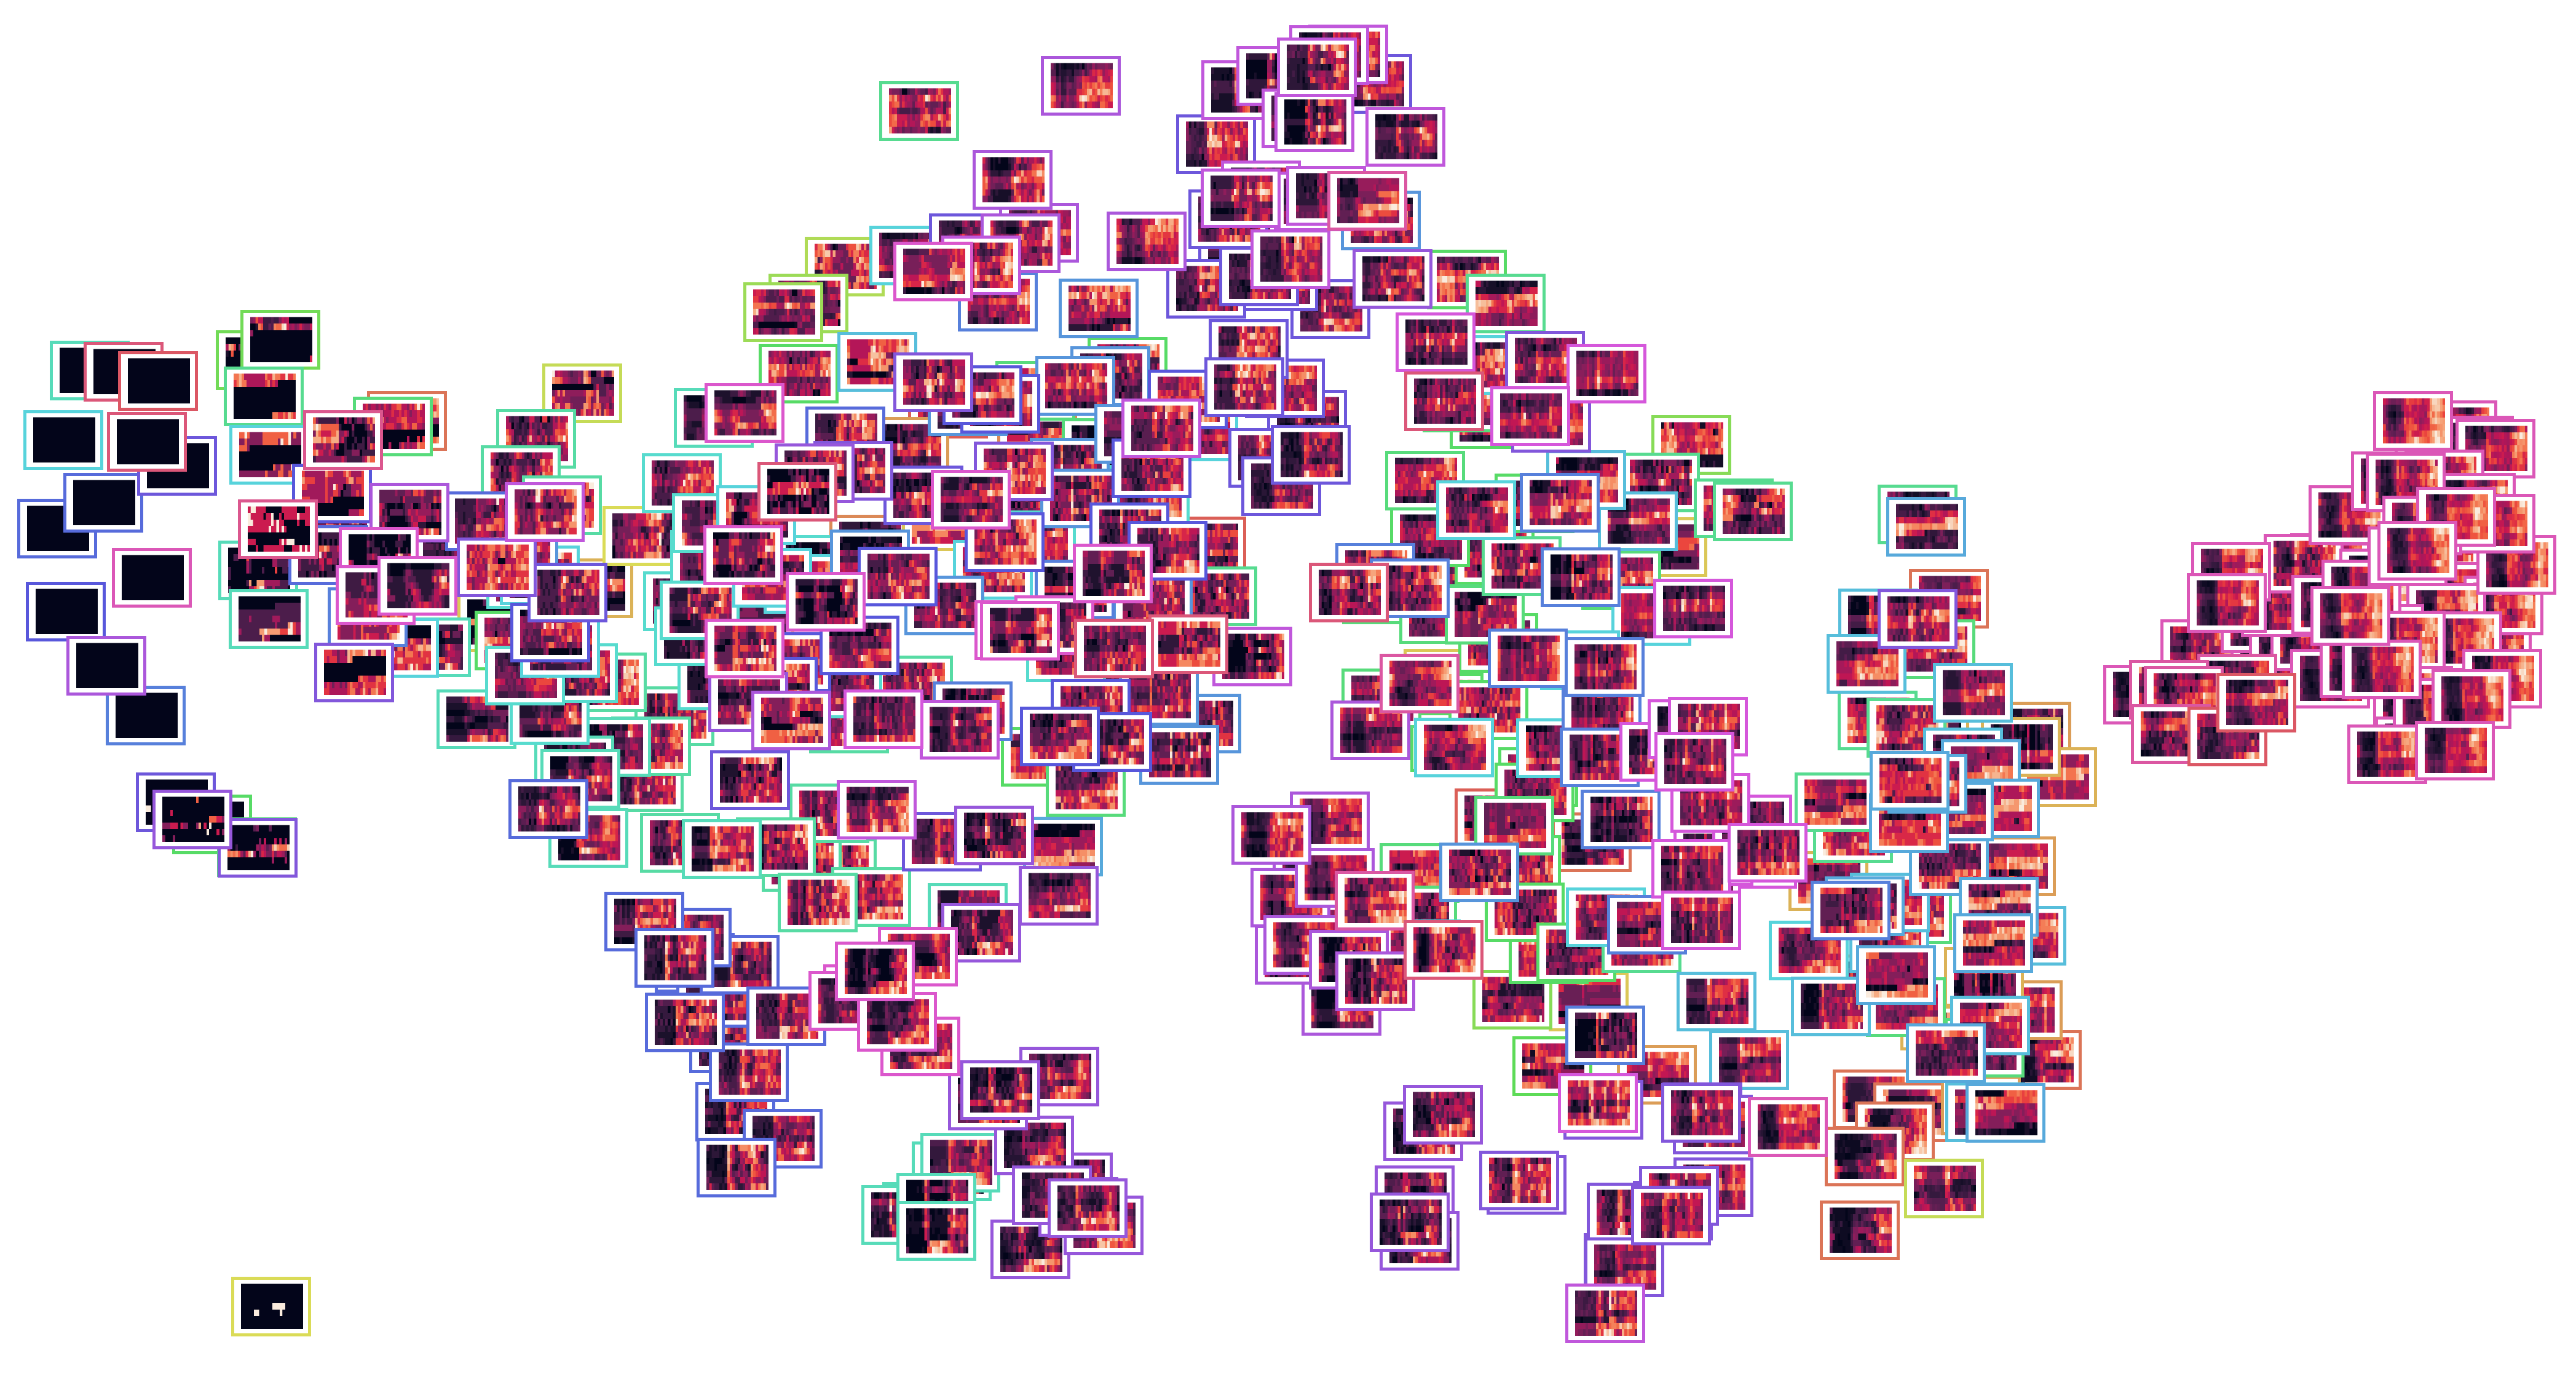
\includegraphics[width=.9\textwidth]{Figures/TSNE/TSNE_per_building/img_scatter_per_building.png}
	\label{fig:tsne_pb_img_scatter_allall}
	\par
	\par\footnotesize{Full resolution figure: \url{https://github.com/jenkoj/msc/tree/main/Figures/TSNE/TSNE_per_building/img_scatter_per_building.png}}
\end{figure}


Figure \ref{fig:tsne_pb_img_scatter_allall} displays the LP for each sample. 
T-SNE provides an intuition of how LPs are connected in higher-dimensional space, and through analysis, we can find clusters with similar usage patterns.
Figure \ref{fig:tsne_pb_img_scatter_allall} shows that the left side has mostly samples with little activity, and the right side has more activity.
When looking at Figure \ref{fig:tsne_scatter_non_norm_all}, we can observe a clear pink colored cluster of LPs from UKDALE 1 and UKDALE 2, which contain plenty of appliances and may explain why they have many activators.
Some less obvious clusters formed in the bottom section for REFIT buildings 2, 3, 5, 6, 4 and 8. 
A significant observation is that LPs closer together have more similar consumption throughout every month.
By measuring the distance between LPs of the same building we can estimate the strength of the household's routine. 

There are no recognizable patterns in the central part of the plot. 
Since there are no patterns, such LPs do not form clusters. 
The reason behind non-recognizable patterns is possibly because appliances like fridges contributed the majority of activations, which are not affected by the dweller, leading to random activations.
Similarly, there are no clusters in the far-left part of the plot because those profiles lack enough information to distinguish them. 

Even though the activations of LPs contained non-normalized activations, some clusters of buildings are quite close to each other.
Here we have to keep in mind the fact that through current presentations we can only observe usage patterns and not usage intensity, which was used as an input to t-SNE
This implies that these buildings have similar usage intensities but not necessarily usage patterns.
We can confirm this, by looking at Figure \ref{fig:tsne_pb_img_scatter_allall}, where it is hard to find what similarities between buildings and clusters that are close together.


% TODO you can write about activation intensify scaler. Max abs is note useful, since most of them would be dark
% We would need some kind of lgaritmic scaling, otherwirse buildings with little appliances would be completley dark and buildings with many appliances completly brihht.
% Either way, presenting these LPs is a hard task

%Efficiently presenting activation intensity is a hard task.
%if we would simply scale all LPs using max-abs scaler, we would be left with some LPs being completely dark and onthers completely white.
%To fix this issue we would have to introduce some kind of logarithmic scaling 

\subsubsection{Normalized LPs}

The issue mentioned in the previous Subsection \ref{ssec:res_pb_lp} can be addressed by normalizing the data between 0 and 1 as mentioned in methodology Section \ref{ssec:norm}.
The normalization should enable t-SNE to focus on finding similarities between the usage patterns.

Figure \ref{fig:tsne_pb_scatter_all_all} illustrates how normalization affects the algorithm.
By comparing Figures \ref{fig:tsne_scatter_non_norm_all} and \ref{fig:tsne_pb_scatter_all_all}, we can observe that the samples in the latter are much closer to each other, while still retaining the individual clusters.
This outcome is expected because normalization removes information regarding the number of appliances in the building.
With a reduced amount of information, LPs become more similar, and therefore clusters are closer together.

\begin{figure}[H]
	\centering
	\caption{Projection of normalized per-building LPs}
	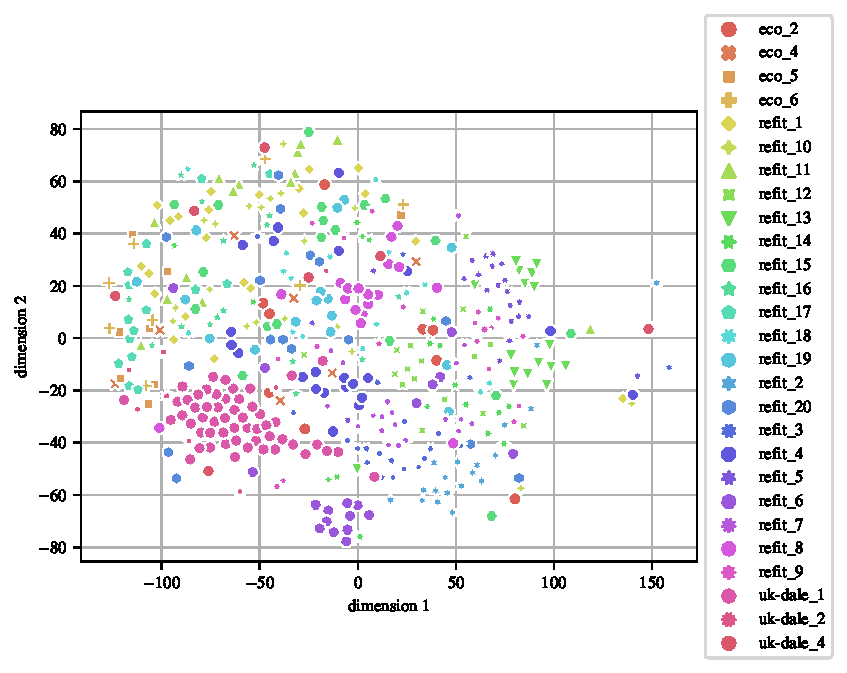
\includegraphics[]{Figures/TSNE/TSNE_per_building/scatter_per_building_norm.pdf}
	\label{fig:tsne_pb_scatter_all_all}
	\par
	\par\footnotesize{Full resolution figure: \url{https://github.com/jenkoj/msc/tree/main/Figures/TSNE/TSNE_per_building/scatter_per_building_norm.pdf}}
\end{figure}

When observing the LPs in Figure \ref{fig:tsne_pb_img_norm_scatter_allall}, we can confirm that similar clusters are closer together.
In this case, the input of the algorithm was the same as our perception of the LPs.
Upon closer look, we can see a gradual and smooth change in patterns as we move across the plot.
If we recall from before that was not the case in Figure \ref{fig:tsne_pb_img_scatter_allall} where we were analyzing non-normalized LPs.
This observation is important, as it is visual proof, that normalization did help the t-SNE to focus on the usage patterns.
% Figure \ref{fig:tsne_pb_img_norm_scatter_allall} presents only the main cluster of samples.
% Since the smaller cluster presents mostly low entropy data, it was cut out. 
% If the reader wants to see the samples in the cluster, the very same cluster can be found on the far left in Figure \ref{fig:tsne_pb_img_scatter_allall}.

\begin{figure}[H]
	\centering
	\caption{Projection of normalized per-building LPs with actual samples}
	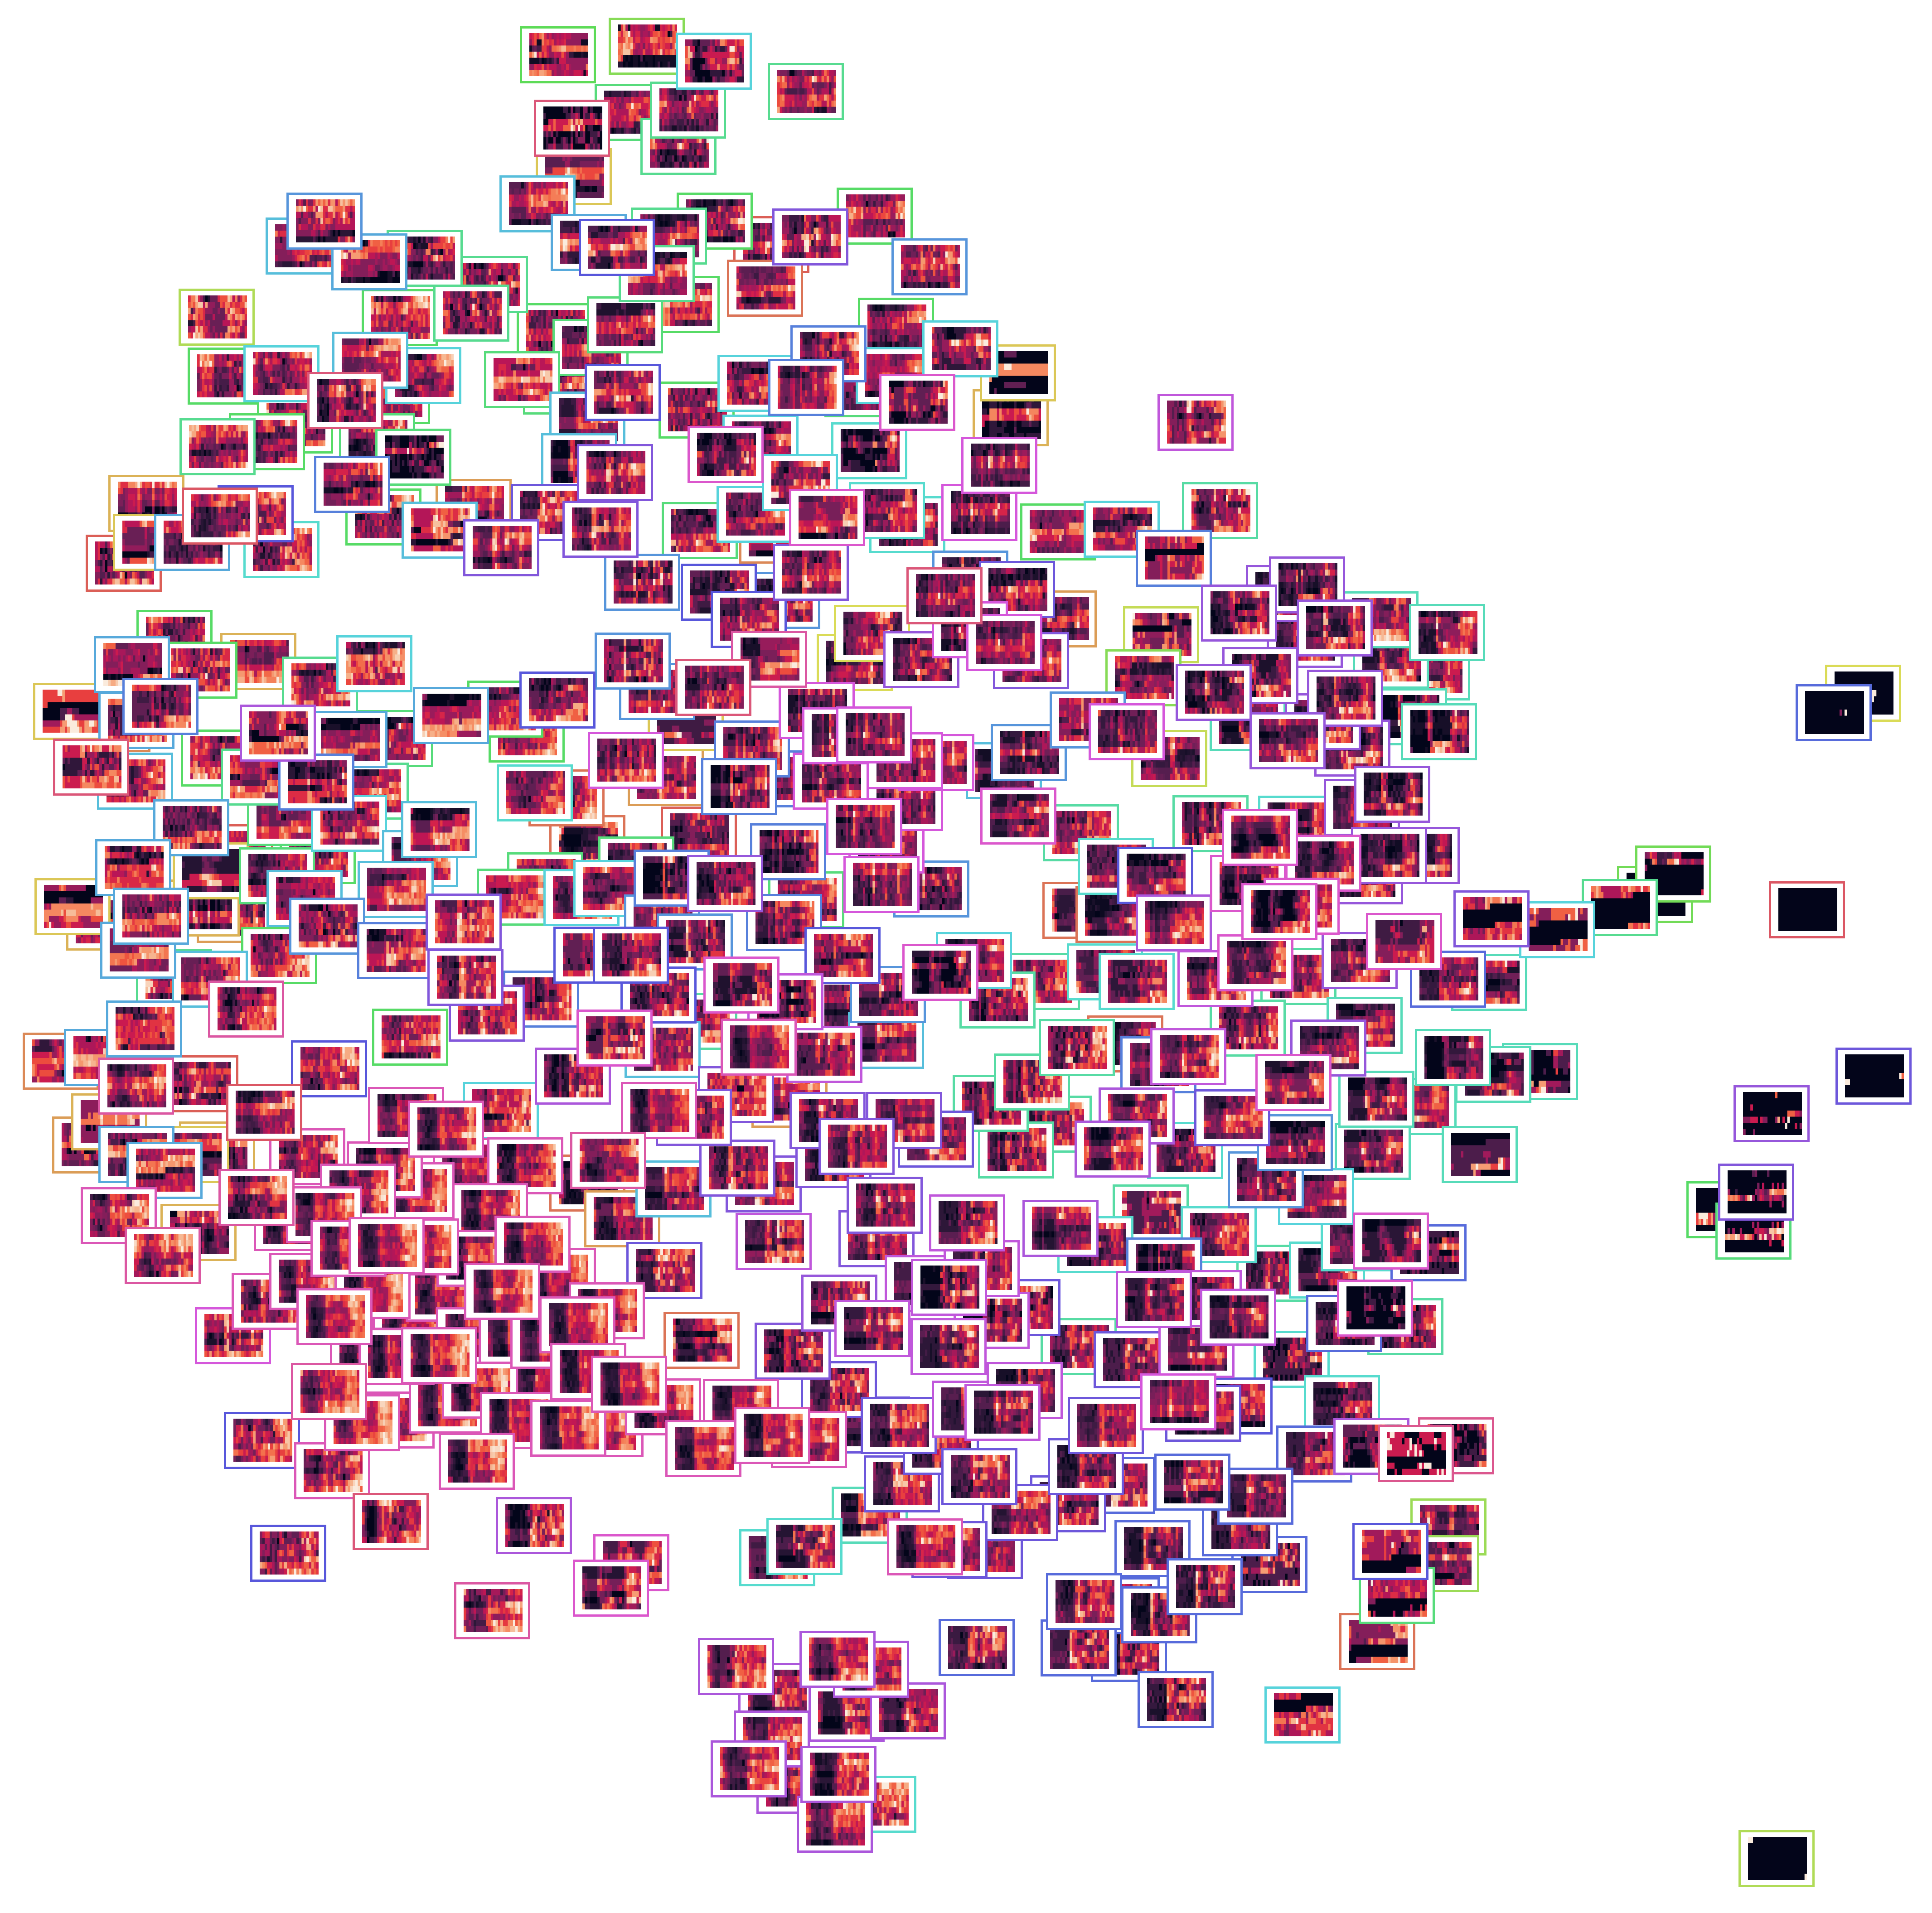
\includegraphics[width=.9\textwidth]{Figures/TSNE/TSNE_per_building/img_scatter_per_building_norm.png}
	\label{fig:tsne_pb_img_norm_scatter_allall}
	\par
	\par\footnotesize{Full resolution figure: \url{https://github.com/jenkoj/msc/tree/main/Figures/TSNE/TSNE_per_building/img_scatter_per_building_norm.png}}
\end{figure}

Upon closer inspection of Figure \ref{fig:tsne_pb_img_norm_scatter_allall} we can see that the general pattern is that there is less activity during the night with one peak in the morning and evening hours.
Some buildings are more active during the week and again some more during the weekend.
A lot of the data is from UK-DALE 1 colored pink. 
It is possible to see that the building has one big cluster where activations are generally similar, with few outliers, where the pattern completely changed. 
This happens due to events such as vacations, holidays or weather-induced behavioral changes.

The key difference between non-normalized and normalized LPs is that,
non-normalized LPs enable t-SNE to identify similarities in the number of appliances and their usage intensity,
while normalized LPs force t-SNE to focus on similarities in the actual usage pattern.
Normalized LPs provide information about when appliances are likely to be used throughout the day, while non-normalized LPs provide insight into the magnitude of appliance usage.

Based on the above observations, we could say that usage patterns are more similar than the number of activations across buildings.
%% TODO finish with a conclusion
\subsection{Per-Appliance}

We can use per-appliance LPs to examine how different appliances 
are used in a single building, how a single appliance is being used across other buildings or how many appliances are being used in many buildings.
Per appliance LPs are built using sub-meter data, meaning each LP should present each appliance.

\subsubsection{Single Appliance Over Many Buildings}

Using one appliance and the building as a label,
allows us to examine how the same type of appliance is being used across different buildings.

Fridges are generally a bad indicator when it comes to user behavior since the user does not affect its operation. 
The only case when the user interacts with it is when opening the door and turning on the light inside. 
Usually, this event is dwarfed by the activations of a compressor. 
This also means that the usage pattern should be the same across all buildings. 
This can be seen in Figure \ref{fig:tsne_pa_scatter_all_fridge}, 
where apart from REFIT buildings 1 and 11, there are no clusters.


\begin{figure}[H]
	\centering
	\caption{Projection of fridge LPs for various buildings}
	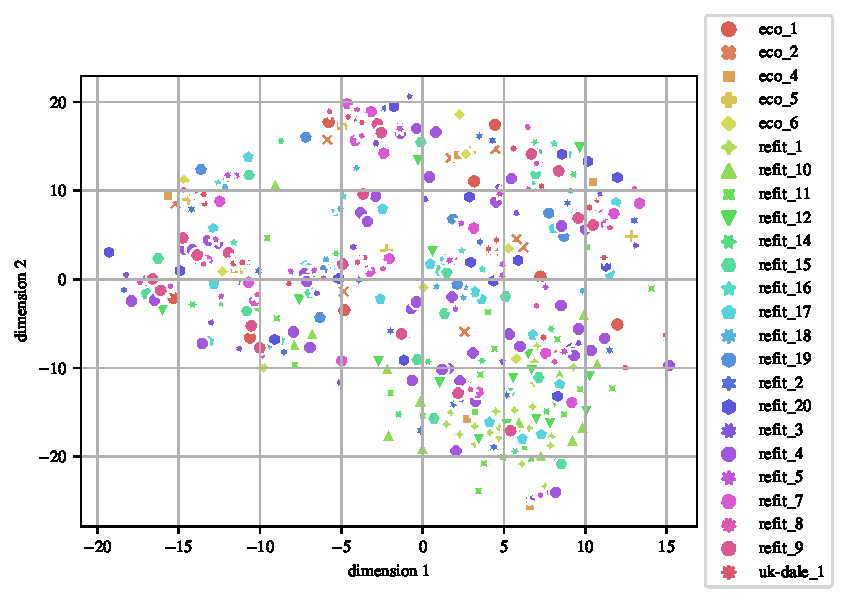
\includegraphics[]{Figures/TSNE/TSNE_per_appliance/scatter_refit_fridge_freeezer_fridge_freezer.pdf}
	\label{fig:tsne_pa_scatter_all_fridge}
	\par
	\par\footnotesize{Full resolution figure: \url{https://github.com/jenkoj/msc/tree/main/Figures/TSNE/TSNE_per_appliance/scatter_refit_fridge_freeezer_fridge_freezer.pdf}}
\end{figure}

Figure \ref{fig:tsne_pa_img_scatter_all_fridge} Shows mostly bright images, apart from a few outliers.
LPs scattered in a circle are generally less dynamic than the ones at the bottom.
Figure \ref{fig:tsne_pa_img_scatter_all_fridge} is a good example of how LPs with little to no human interaction, can look a lot different. 
This could be due to different makes of the appliances, malfunctions of the appliance or the meter measuring it.

\begin{figure}[H]
	\centering
	\caption{Projection of fridge LPs for various buildings with actual samples}
	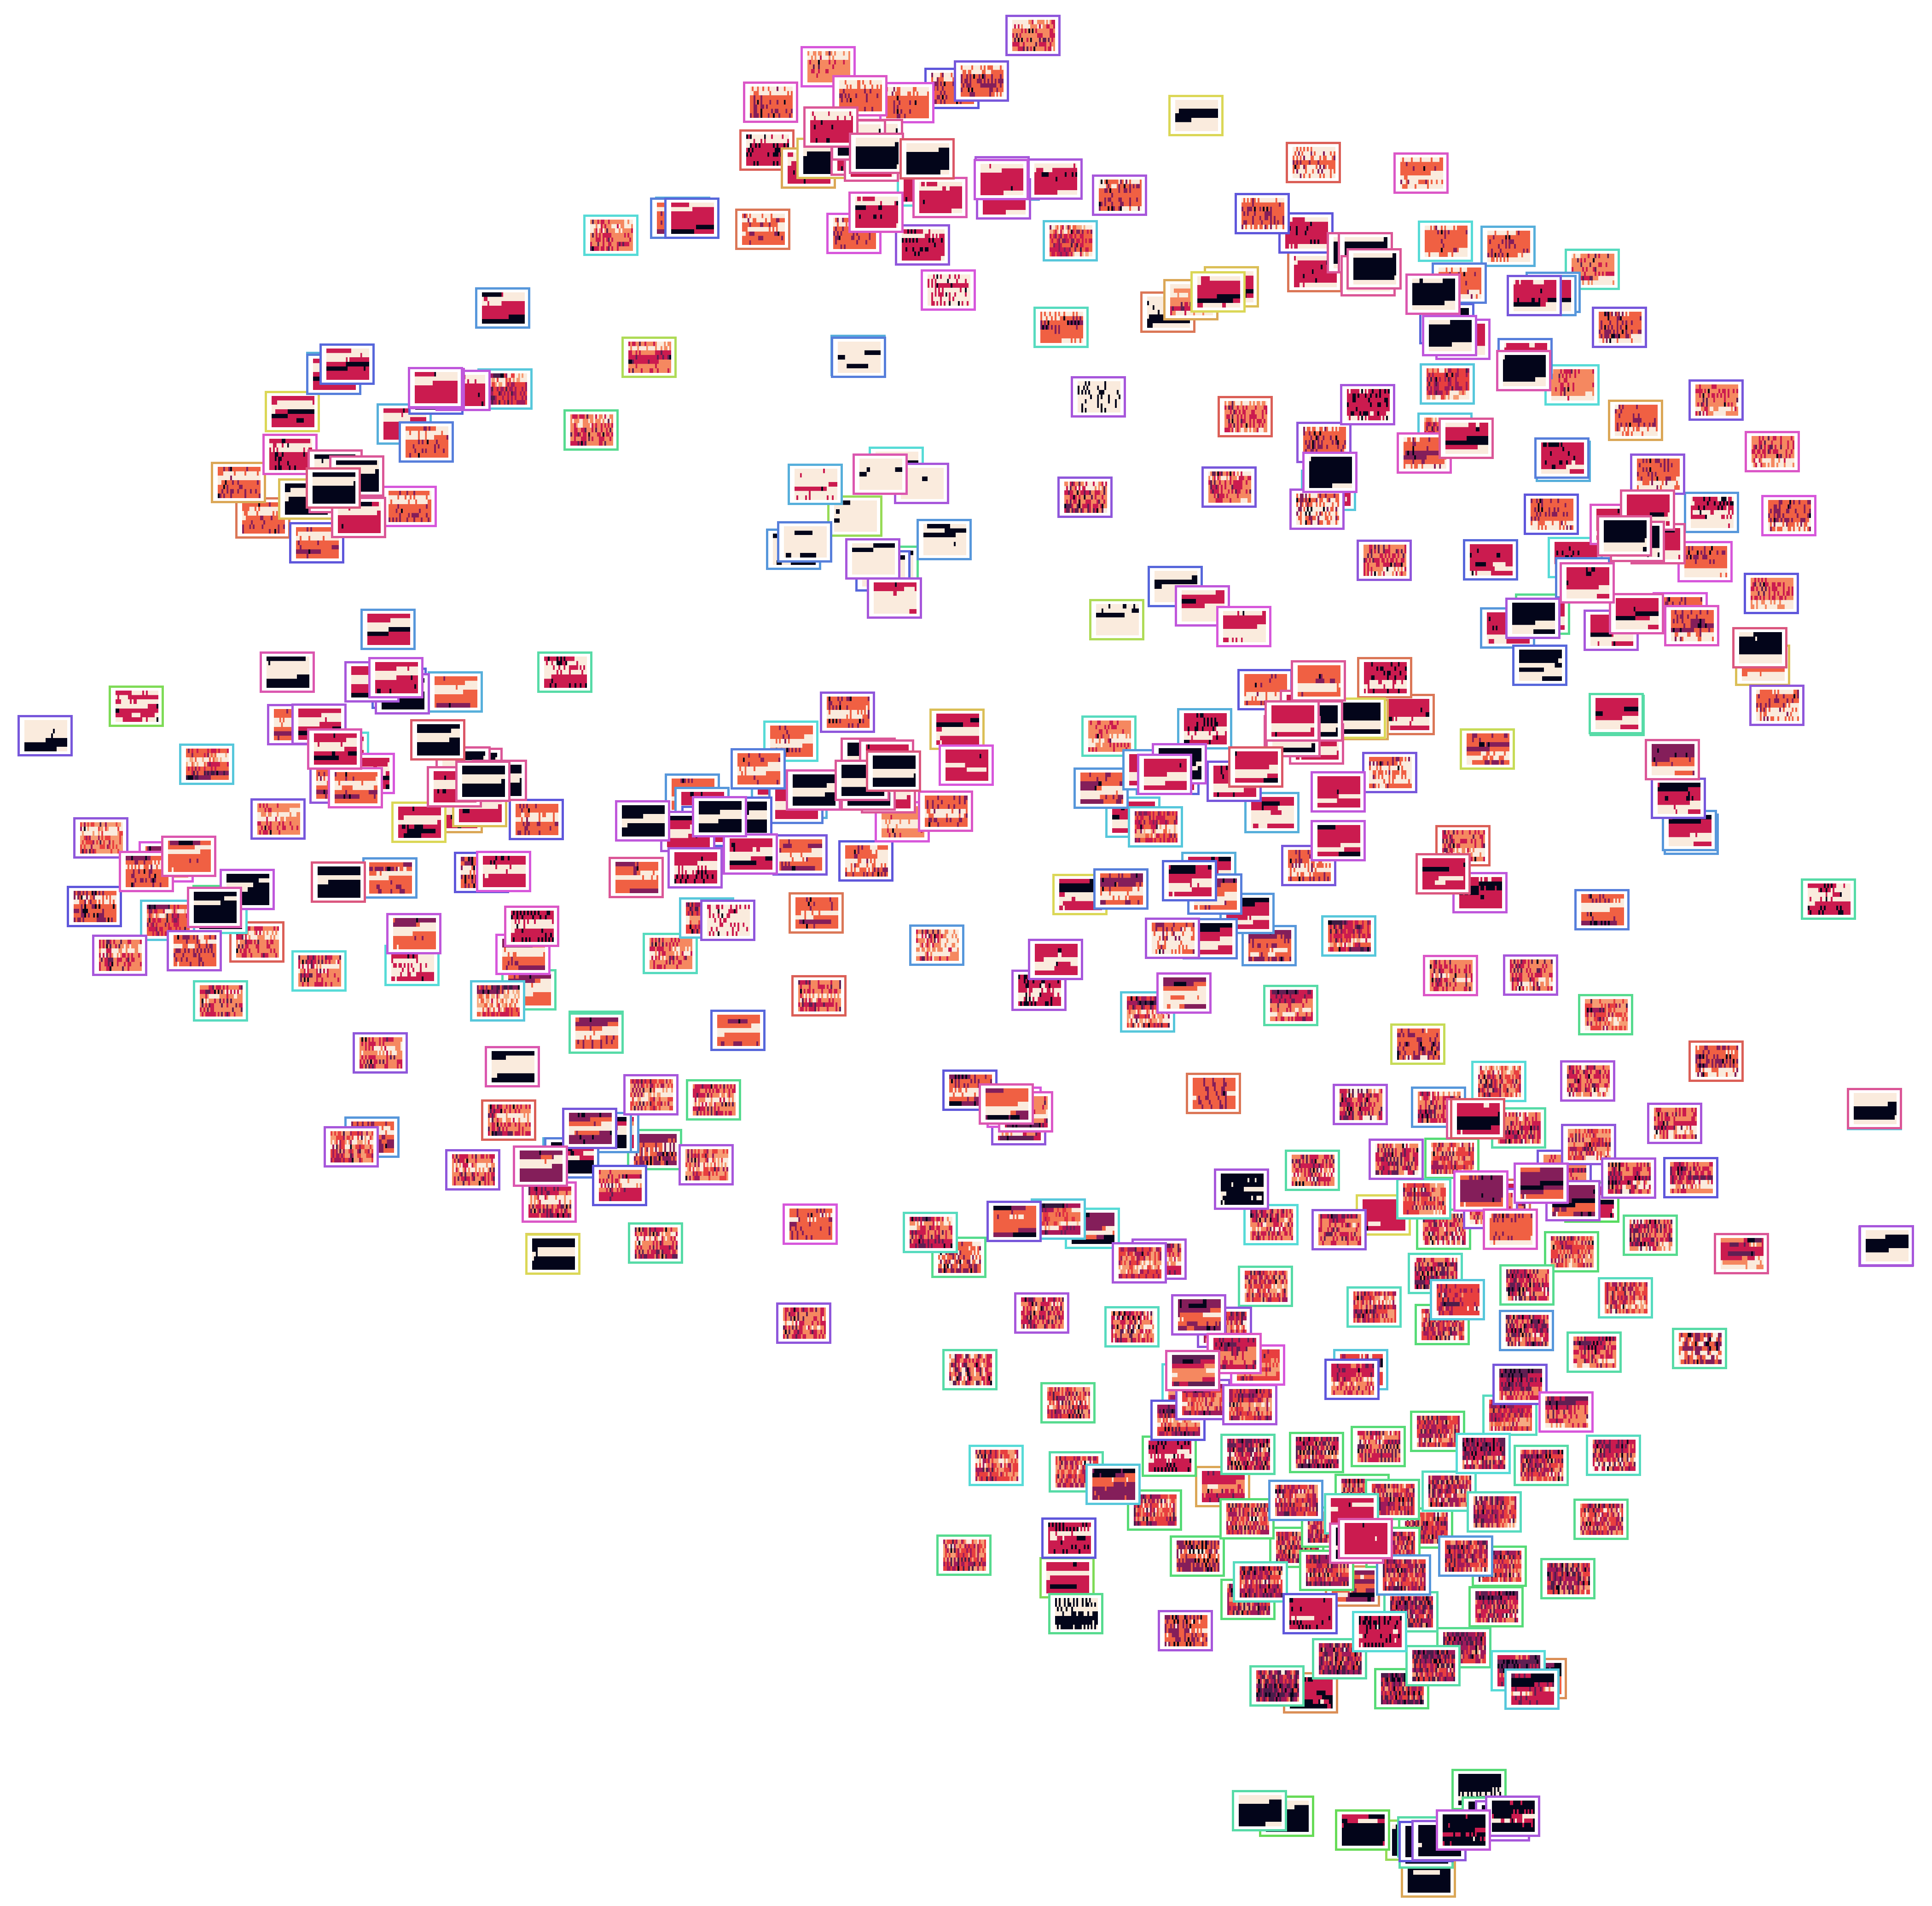
\includegraphics[width=.9\textwidth]{Figures/TSNE/TSNE_per_appliance/img_scatter_refit_fridge_freeezer_fridge_freezer.png}
	\label{fig:tsne_pa_img_scatter_all_fridge}
	\par
	\par\footnotesize{Full resolution figure: \url{https://github.com/jenkoj/msc/tree/main/Figures/TSNE/TSNE_per_appliance/img_scatter_refit_fridge_freeezer_fridge_freezer.png}}
\end{figure}

Figure \ref{fig:tsne_pa_scatter_all_kettle} shows how,
compared to fridges, kettles have many clear clusters that are spaced out between each other. 
This could mean that every household uses a kettle a bit differently.
These clusters are a good example where we can observe how strong is a routine of a user.
The closer together the samples in individual clusters are, the higher the routine since samples are more similar to each other.

\begin{figure}[H]
	\centering
	\caption{Projection of kettle LPs for various buildings}
	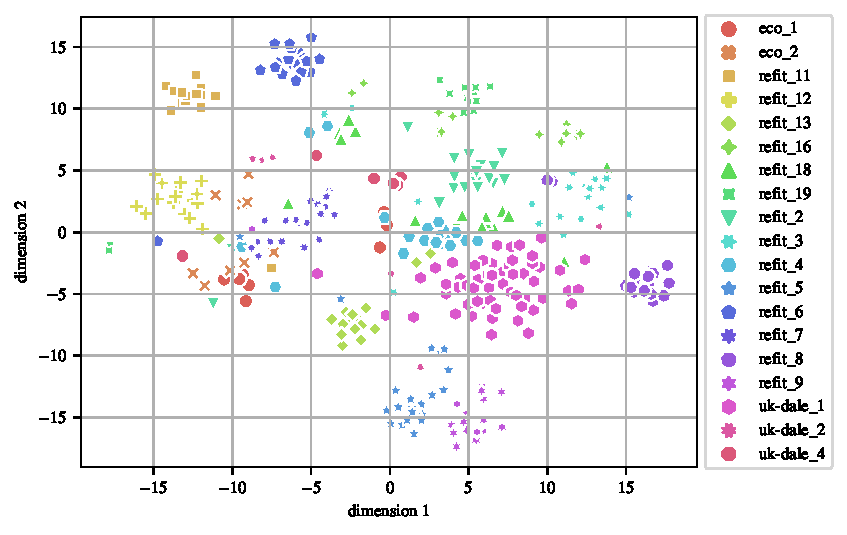
\includegraphics[]{Figures/TSNE/TSNE_per_appliance/scatter_refit_kettle.pdf}
	\label{fig:tsne_pa_scatter_all_kettle}
	\par
	\par\footnotesize{Full resolution figure: \url{https://github.com/jenkoj/msc/tree/main/Figures/TSNE/TSNE_per_appliance/scatter_refit_kettle.pdf}}
\end{figure}

Figure \ref{fig:tsne_pa_img_scatter_all_kettle} shows us that images on the lower part 
of the plot contain less activity than the others. 
LPs that are closer together have more similar activation patterns.
Similar activation patterns are caused by similar behavior, which is essentially a routine.
This means that this projection could be used to calculate how much a behavior variates in time for each building.
This could be calculated by measuring the scattering of samples (variance) for each building.

If we find samples that always activate in the same morning buckets, we would see that they form a straight line on the y-axis.
This is the daily routine. One such example can be seen in Figure \ref{fig:tsne_pa_scatter_all_kettle} in cluster REFIT 5 and REFIT 9, where we can see the lines and the pattern throughout the day. 
Since the routine is present, the samples look more similar and are therefore closer together. 
This does not necessarily mean that the closer the samples higher the routine.
They could also be together in case of "ordered chaos" such as can be seen in Figure \ref{fig:tsne_pa_scatter_all_kettle} for building refit 16 and refit 8 where there is no pattern through the day.
So the scattering is not a precise metric when it comes to the routine, but it gives us a rough idea of its presence.
As mentioned earlier in this chapter the strength of a routine is an important feature that will be used
in Chapter \ref{chapter6}, where we will build an elderly care anomaly detection system.

\begin{figure}[H]
	\centering
	\caption{Projection of kettle LPs for various buildings with actual samples}
	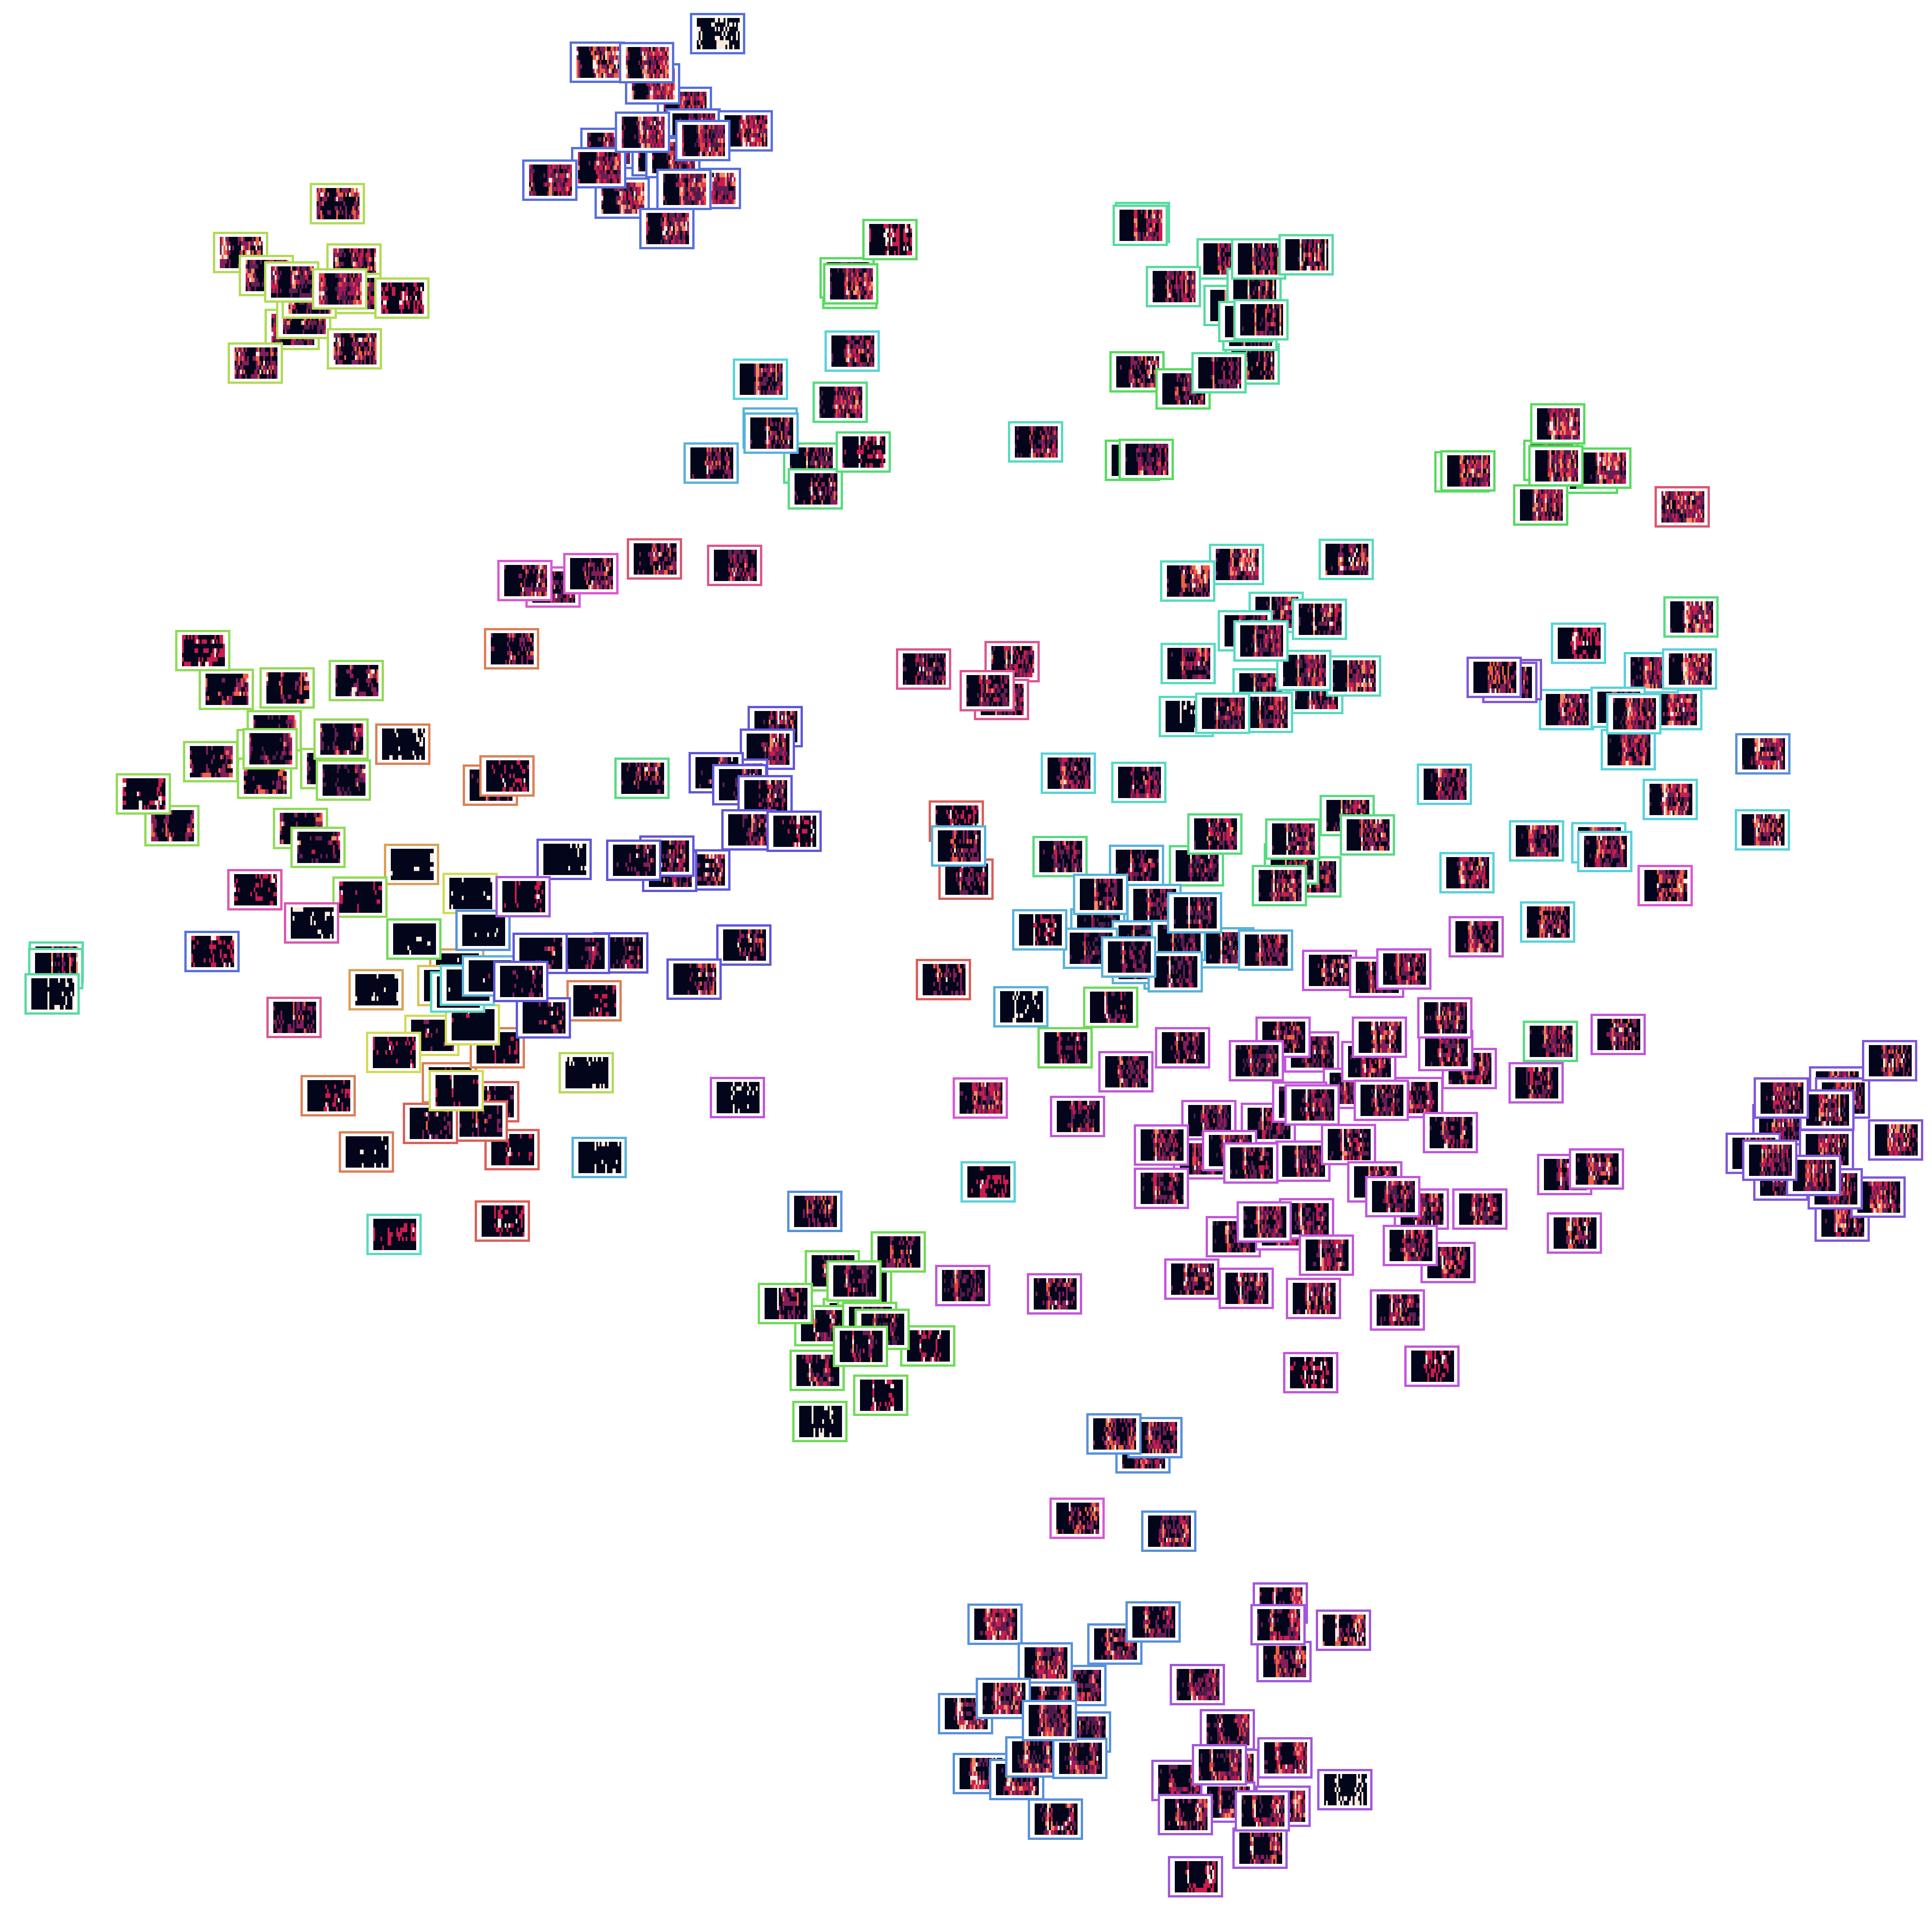
\includegraphics[width=.9\textwidth]{Figures/TSNE/TSNE_per_appliance/img_scatter_refit_kettle.png}
	\label{fig:tsne_pa_img_scatter_all_kettle}
	\par
	\par\footnotesize{Full resolution figure: \url{https://github.com/jenkoj/msc/tree/main/Figures/TSNE/TSNE_per_appliance/img_scatter_refit_kettle.png}}
\end{figure}

% Figure \ref{fig:tsne_pa_scatter_all_microwave} shows that microwaves are again a bit different from the kettle.
% They are more clustered than the fridges, and less than the kettles, even though they are used similarly.
% This could be due to additional electronics such as a clock that are built into
% the appliance. This could lead to some samples being registered as turned on due to 
% a "dark" current. One other difference between the two is that microwave has more than one mode of operation.

% \begin{figure}[H]
% 	\centering
% 	\caption{Projection of microwave LPs for various buildings}
% 	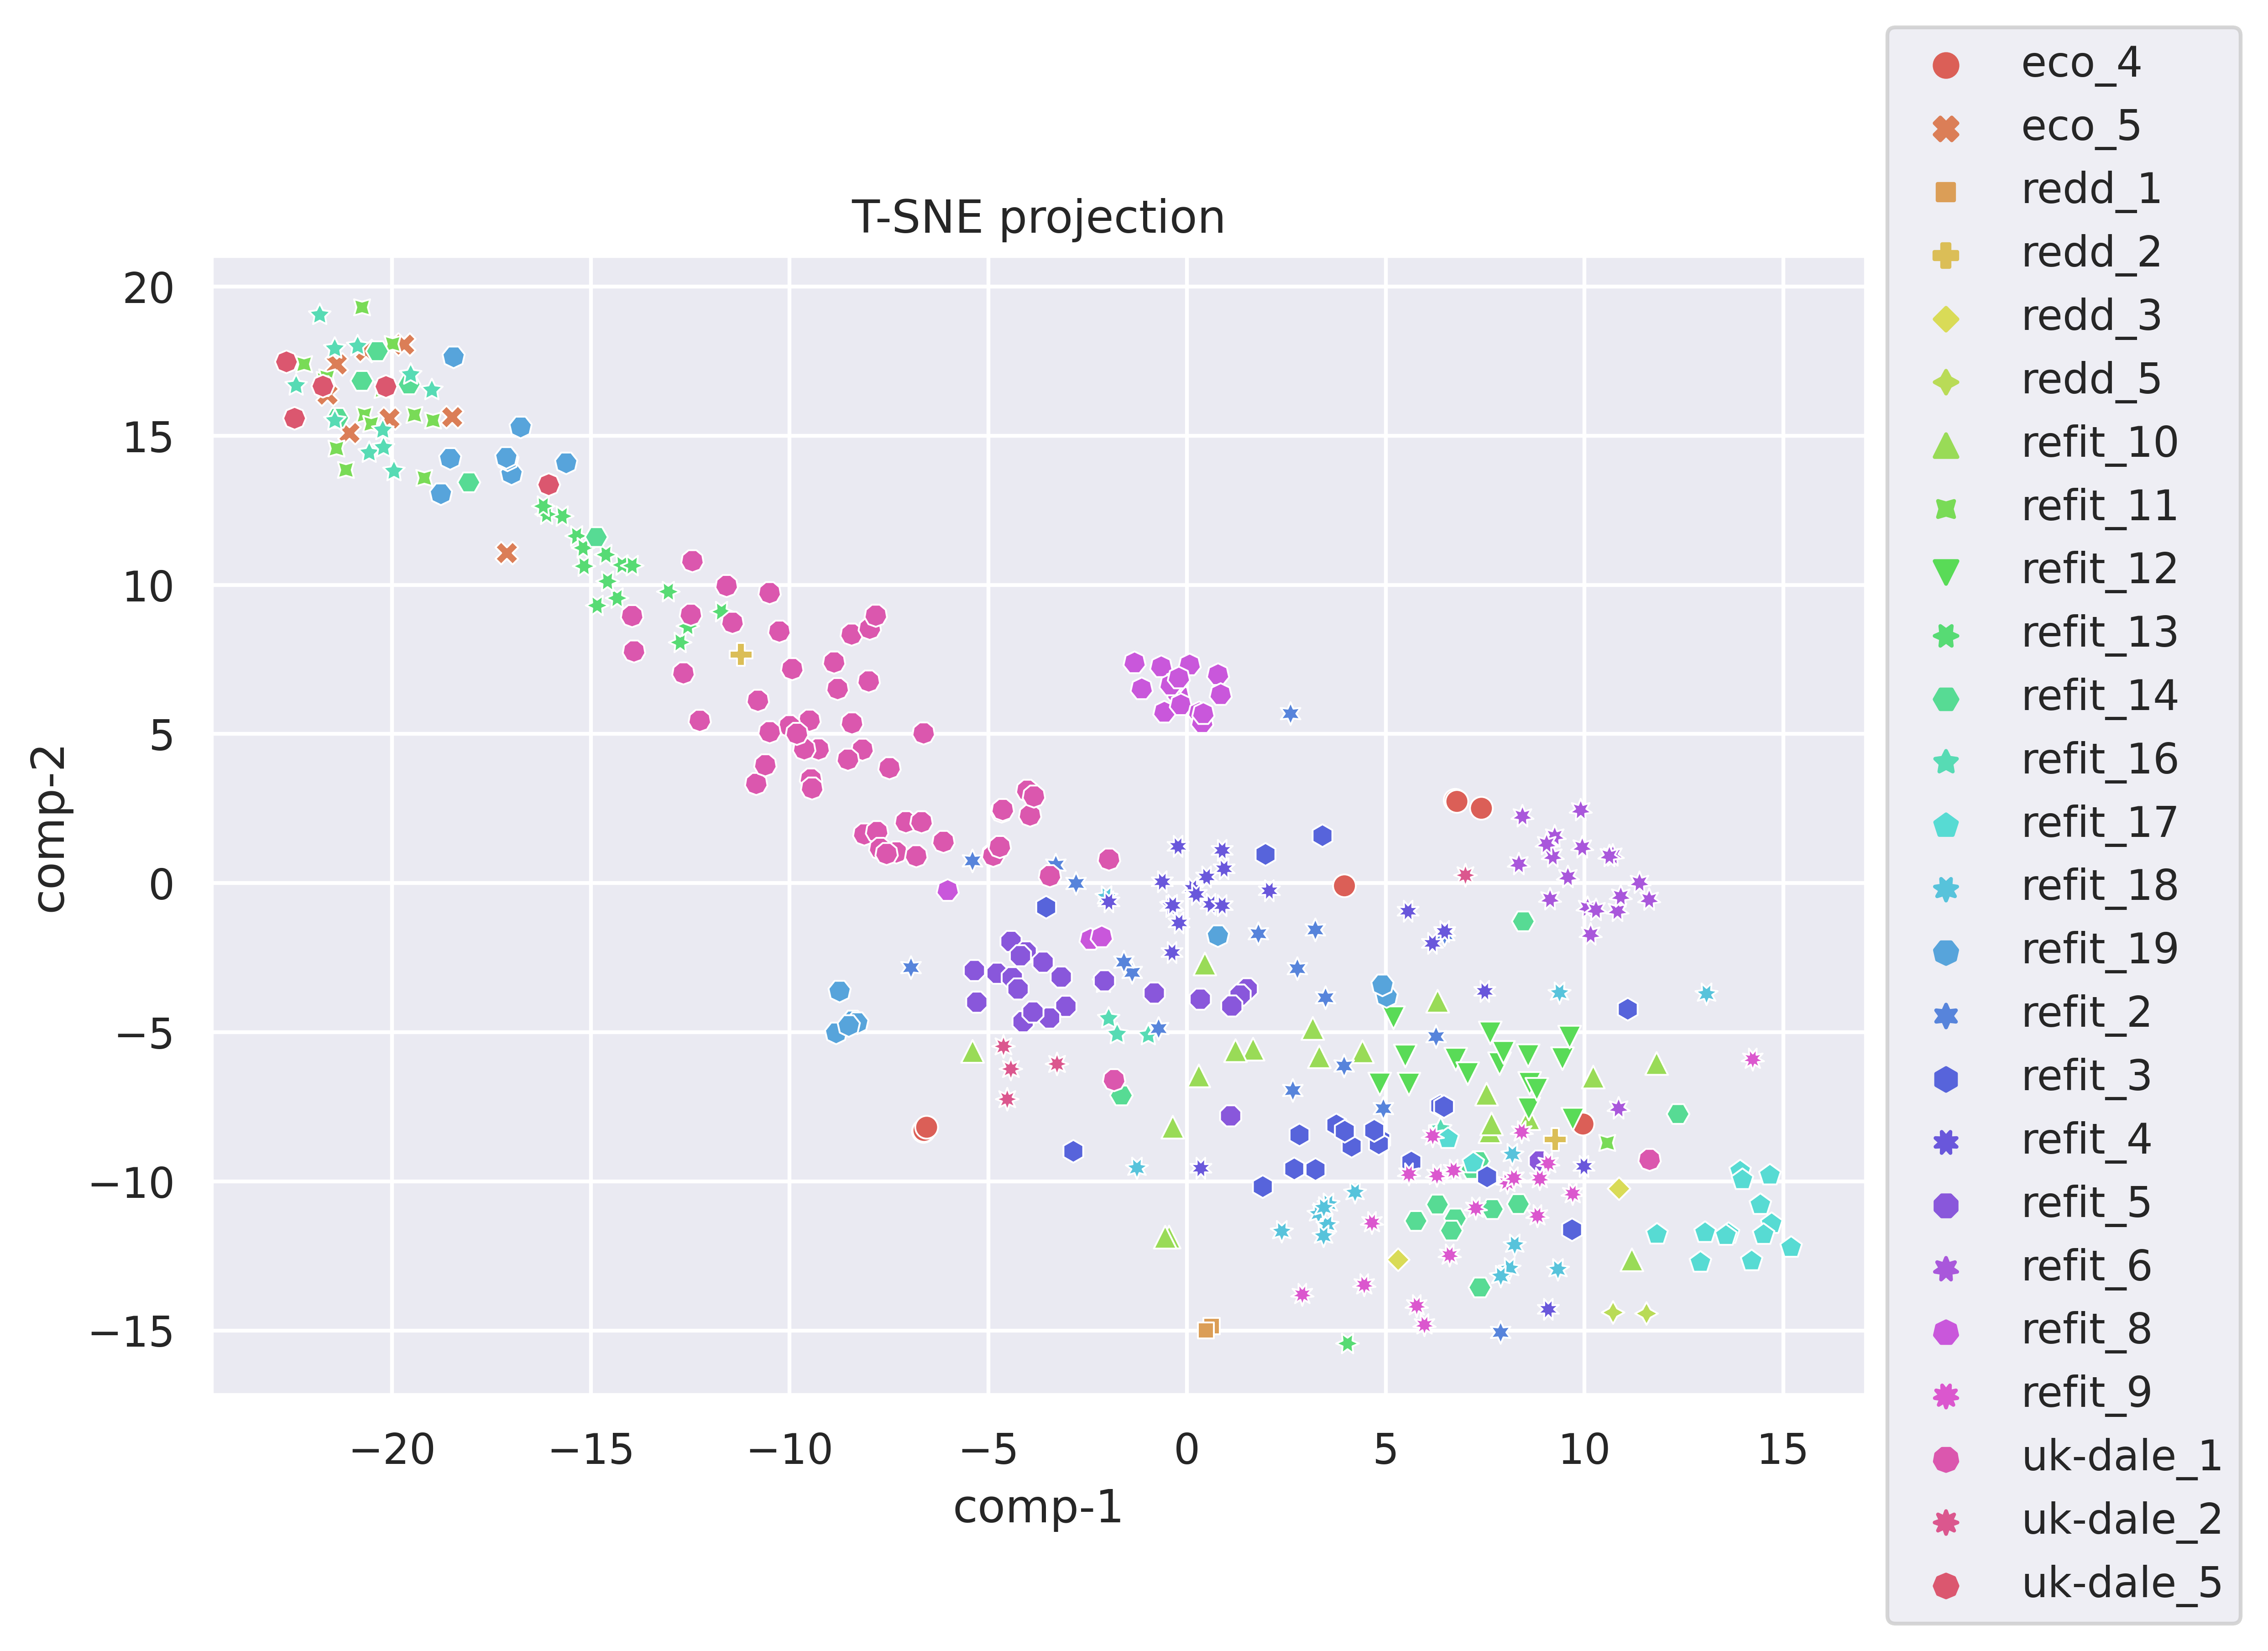
\includegraphics[width=1.2\textwidth]{Figures/TSNE/TSNE_per_appliance/all/scatter_all_microwave.png}
% 	\label{fig:tsne_pa_scatter_all_microwave}
% \end{figure}

% Figure \ref{fig:tsne_pa_img_scatter_all_microwave} shows the faulty samples could be the ones in the upper left part of the plot since they are too bright.
% They do present a pattern, but it is questionable what it presents since it seems like it's turned on during the nighttime. 
% Images at the other end show less lot less activity, which could indicate that
% the household does not use microwaves as much. The most interesting LPs are in the middle of the 
% plot, where it is possible to observe clear activation patterns. 

% \begin{figure}[H]
% 	\centering
% 	\caption{Projection of microwave LPs for various buildings with actual samples}
% 	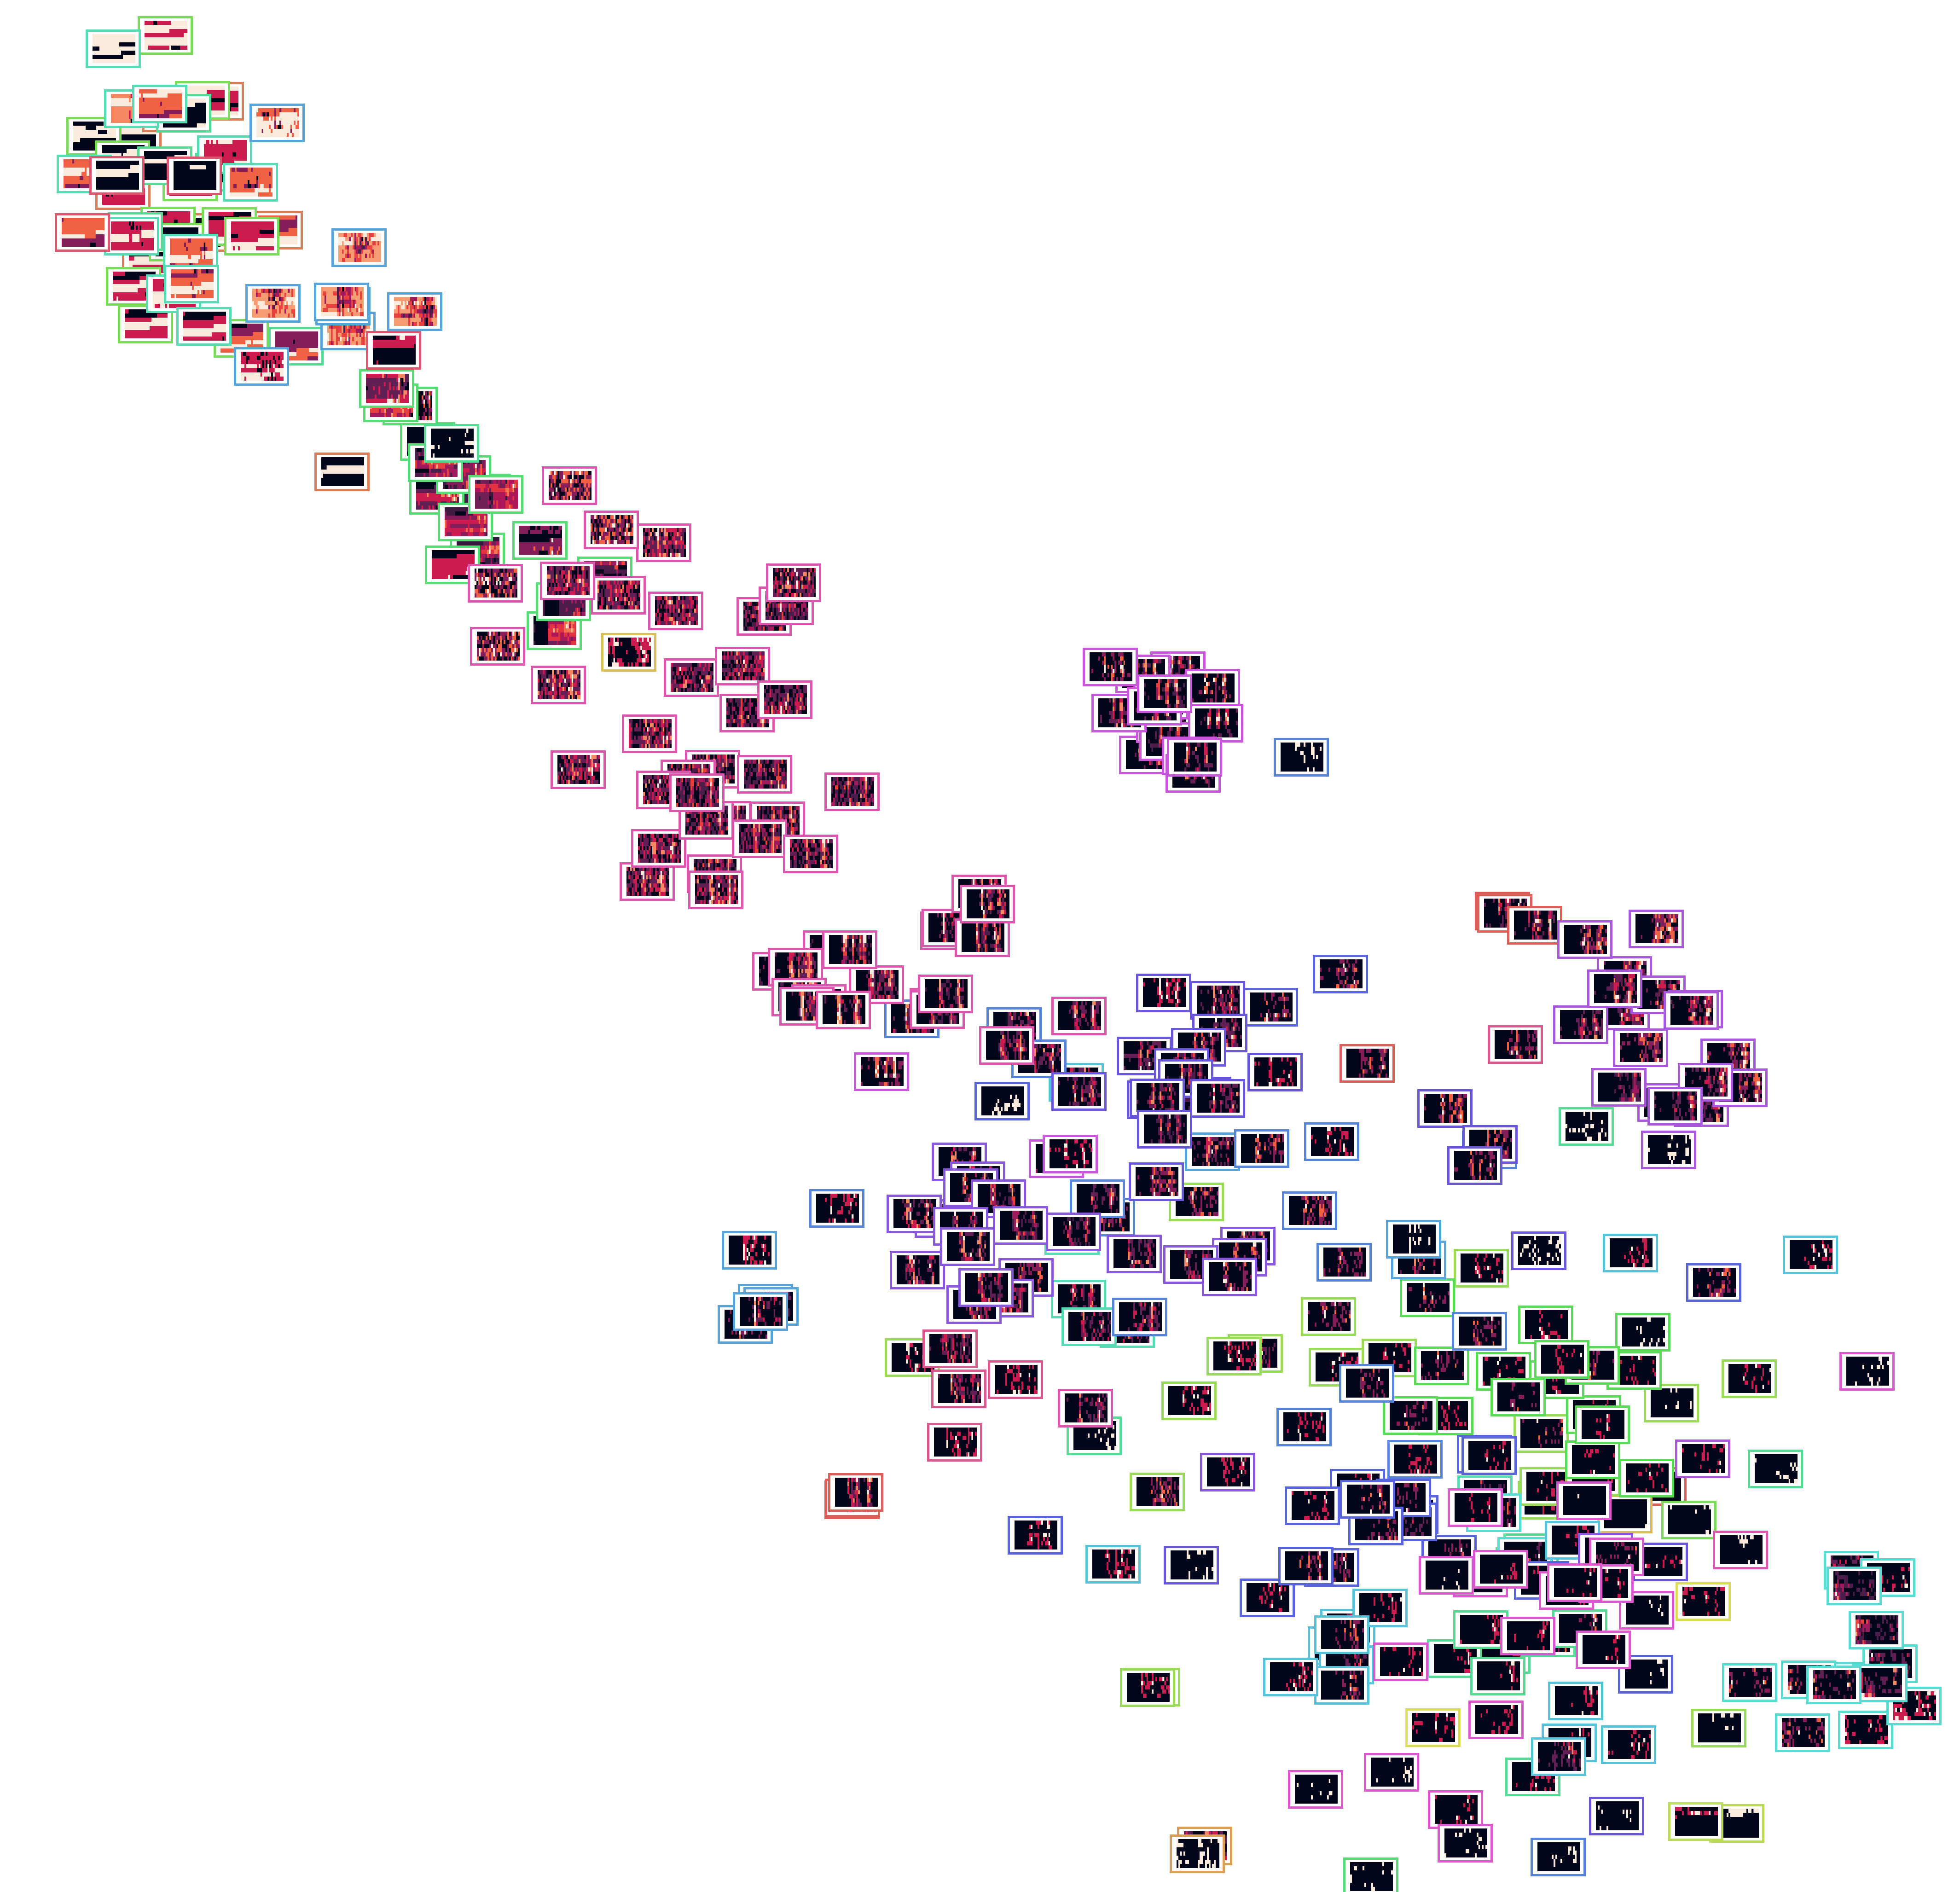
\includegraphics[width=.9\textwidth]{Figures/TSNE/TSNE_per_appliance/all/img_scatter_allmicrowave.png}
% 	\label{fig:tsne_pa_img_scatter_all_microwave}
% \end{figure}

The last per-appliance example is television presented in Figure \ref{fig:tsne_pa_scatter_all_tv}. 
Television was chosen since it is the most commonly occurring appliance.
Interestingly enough, televisions form nice clusters with a few outliers.
Clusters are separated but close together, this could mean that usage patterns across buildings are unique
but not that different from one another. 
The LPs in some clusters are also close to each other, which could also indicate 
a higher routine.

\begin{figure}[H]
	\centering
	\caption{Projection of TV LPs for various buildings}
	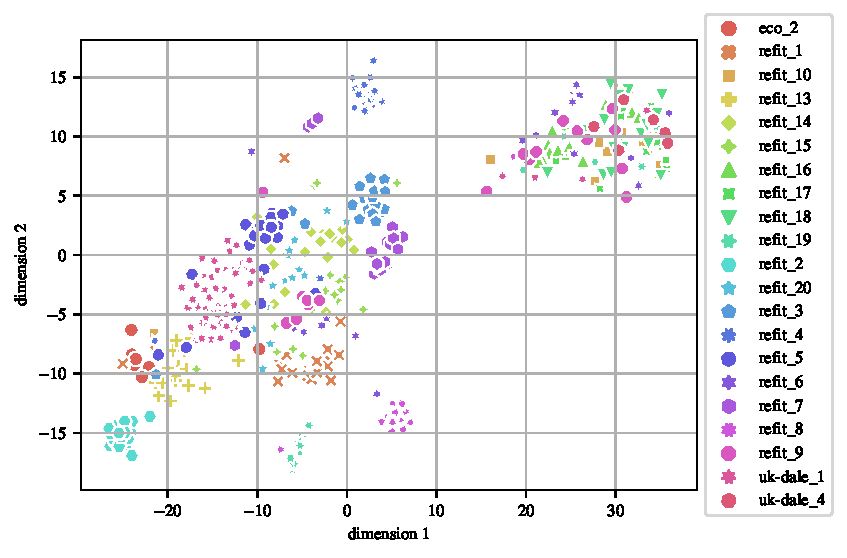
\includegraphics[]{Figures/TSNE/TSNE_per_appliance/scatter_refit_television.pdf}
	\label{fig:tsne_pa_scatter_all_tv}
	\par
	\par\footnotesize{Full resolution figure: \url{https://github.com/jenkoj/msc/tree/main/Figures/TSNE/TSNE_per_appliance/scatter_refit_television.pdf}}
\end{figure}

The images in Figure \ref{fig:tsne_pa_img_scatter_all_tv} prove the fact that outliers' consumption is a lot different.
Again the bright images could be the results of faulty appliances, faulty meters or simply odd behavior.
Figure \ref{fig:tsne_pa_img_scatter_all_tv} also enables us to see that TVs are primarily used 
in the evening hours. Outliers from the main cluster show slightly different behavior. One such 
example is the blue cluster (building REFIT 4), where appliances are mostly used in the morning hours. 
One other interesting observation can be made when looking at the purple cluster. This is the far low cluster for building REFIT 8.
Here, the TV is being consistently used every day in the early morning hours.
This is portrayed as a straight line.
There could be two possible explanations for this.
First is simply a high routine of a user, who turns on the TV every morning to listen to the news.
The other is that the TV updates itself every morning. This is probably not the case since updates do not occur on regular basis.
What is also interesting, is that the very same pattern can be observed in a few other buildings, one example being building REFIT 19.

\begin{figure}[H]
	\centering
	\caption{Projection of TV LPs for various buildings with actual samples.}
	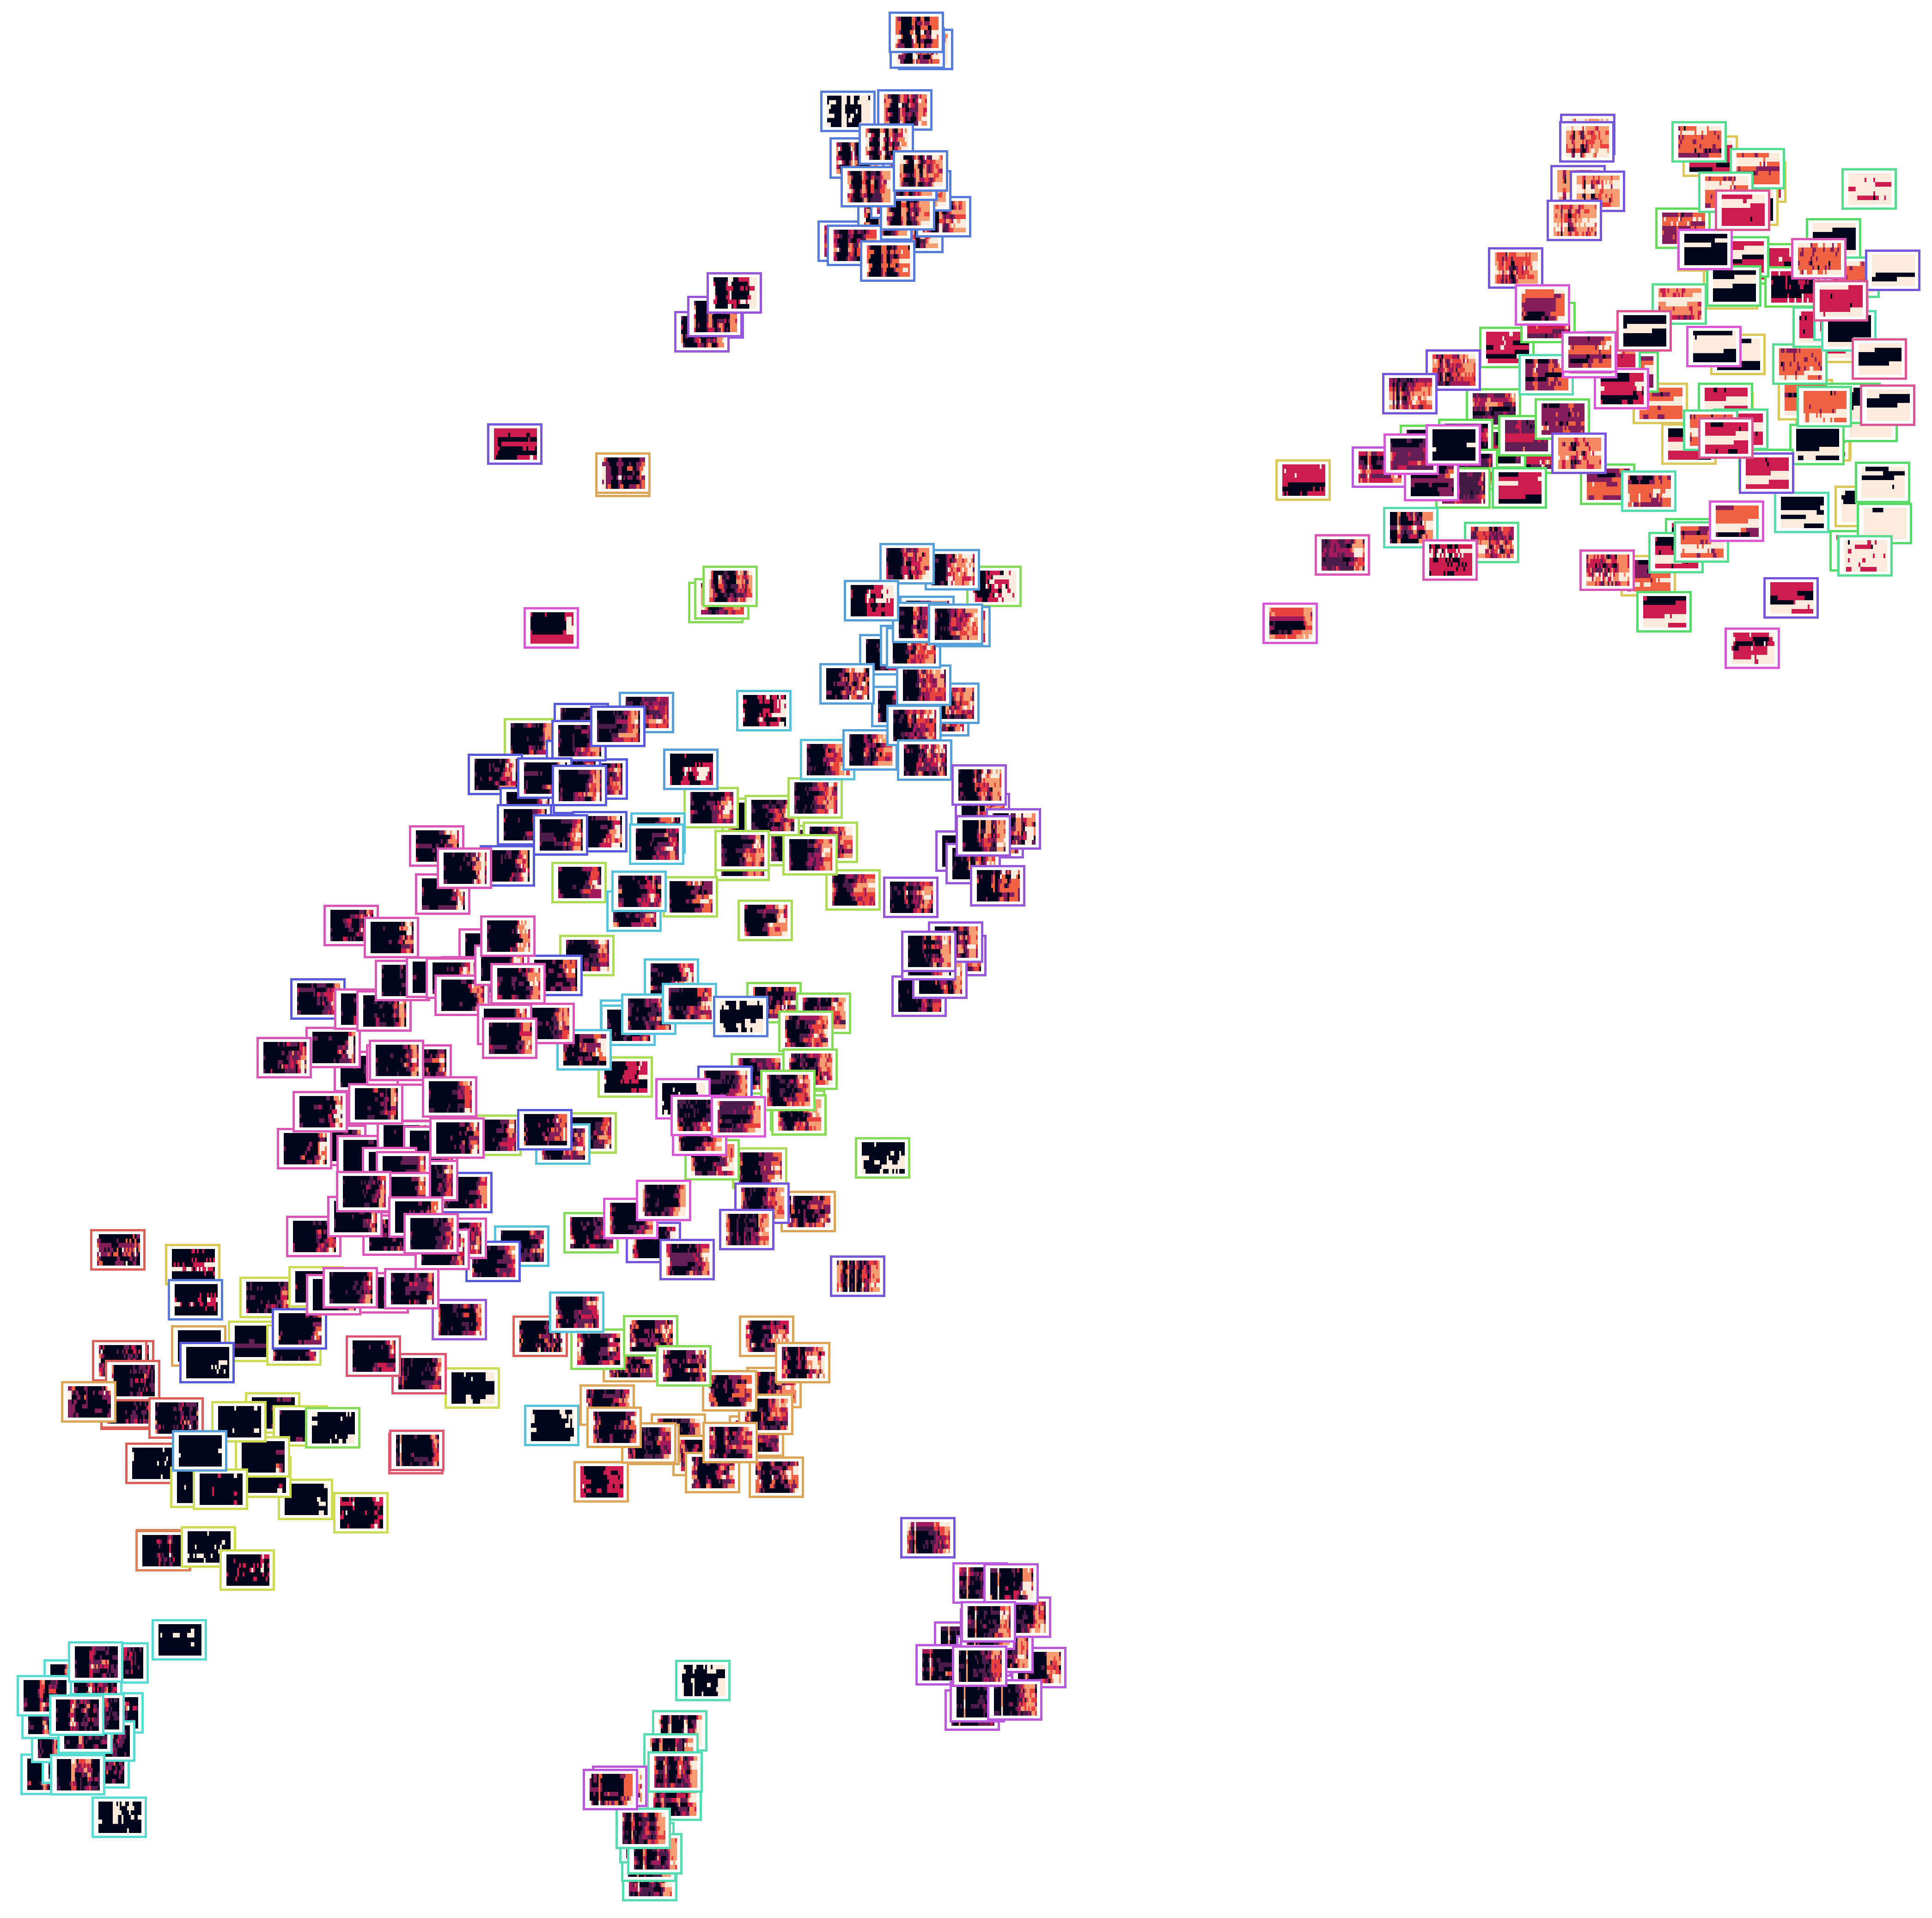
\includegraphics[width=.9\textwidth]{Figures/TSNE/TSNE_per_appliance/img_scatter_refit_television.png}
	\label{fig:tsne_pa_img_scatter_all_tv}
	\par
	\par\footnotesize{Full resolution figure: \url{https://github.com/jenkoj/msc/tree/main/Figures/TSNE/TSNE_per_appliance/img_scatter_refit_television.png}}
\end{figure}

\subsubsection{Per-Appliance LPs - Comparing Appliances}

% Figure \ref{fig:tsne_papb_scatter_all} presents the general picture of where each appliance lays in comparison to the other.
% One obvious issue here is that there are too many appliances, and it is impossible to comprehend the plot.

% \begin{figure}[H]
% 	\centering
% 	\caption{Projection of per-appliance LPs}
% 	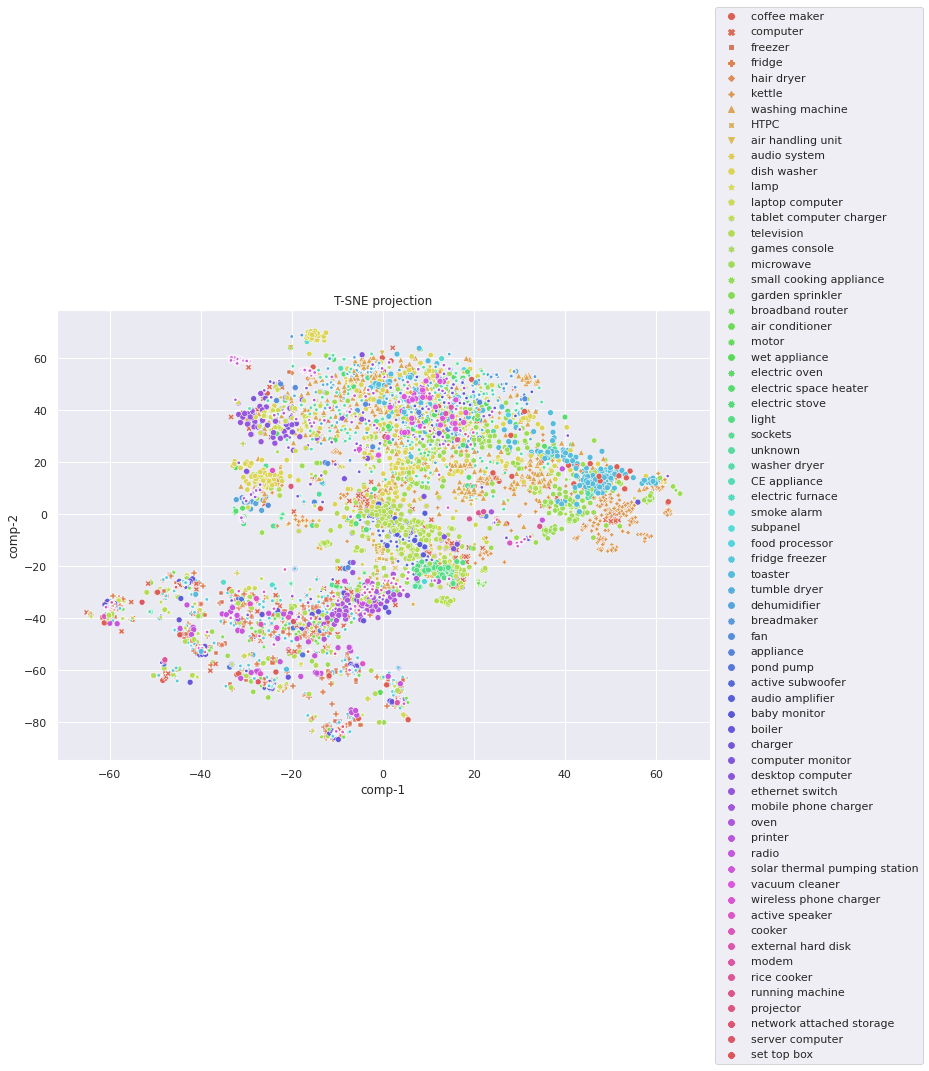
\includegraphics[width=1.2\textwidth]{Figures/TSNE/TSNE_results/all/scatter_all_all_lgimgs.png}
% 	\label{fig:tsne_papb_scatter_all}
% \end{figure}

% The same goes for image presentation in Figure \ref{fig:tsne_papb_img_scatter_all}. 
% We can see, that most active appliances are the ones in the bottom left,
% by moving to the upper right part of the corner, we can see less activity.
% Less activity does not necessarily mean that LPs contain less information about user behavior.

% \begin{figure}[H]
% 	\centering
% 	\caption{Projection of per-appliance LPs with actual samples}
% 	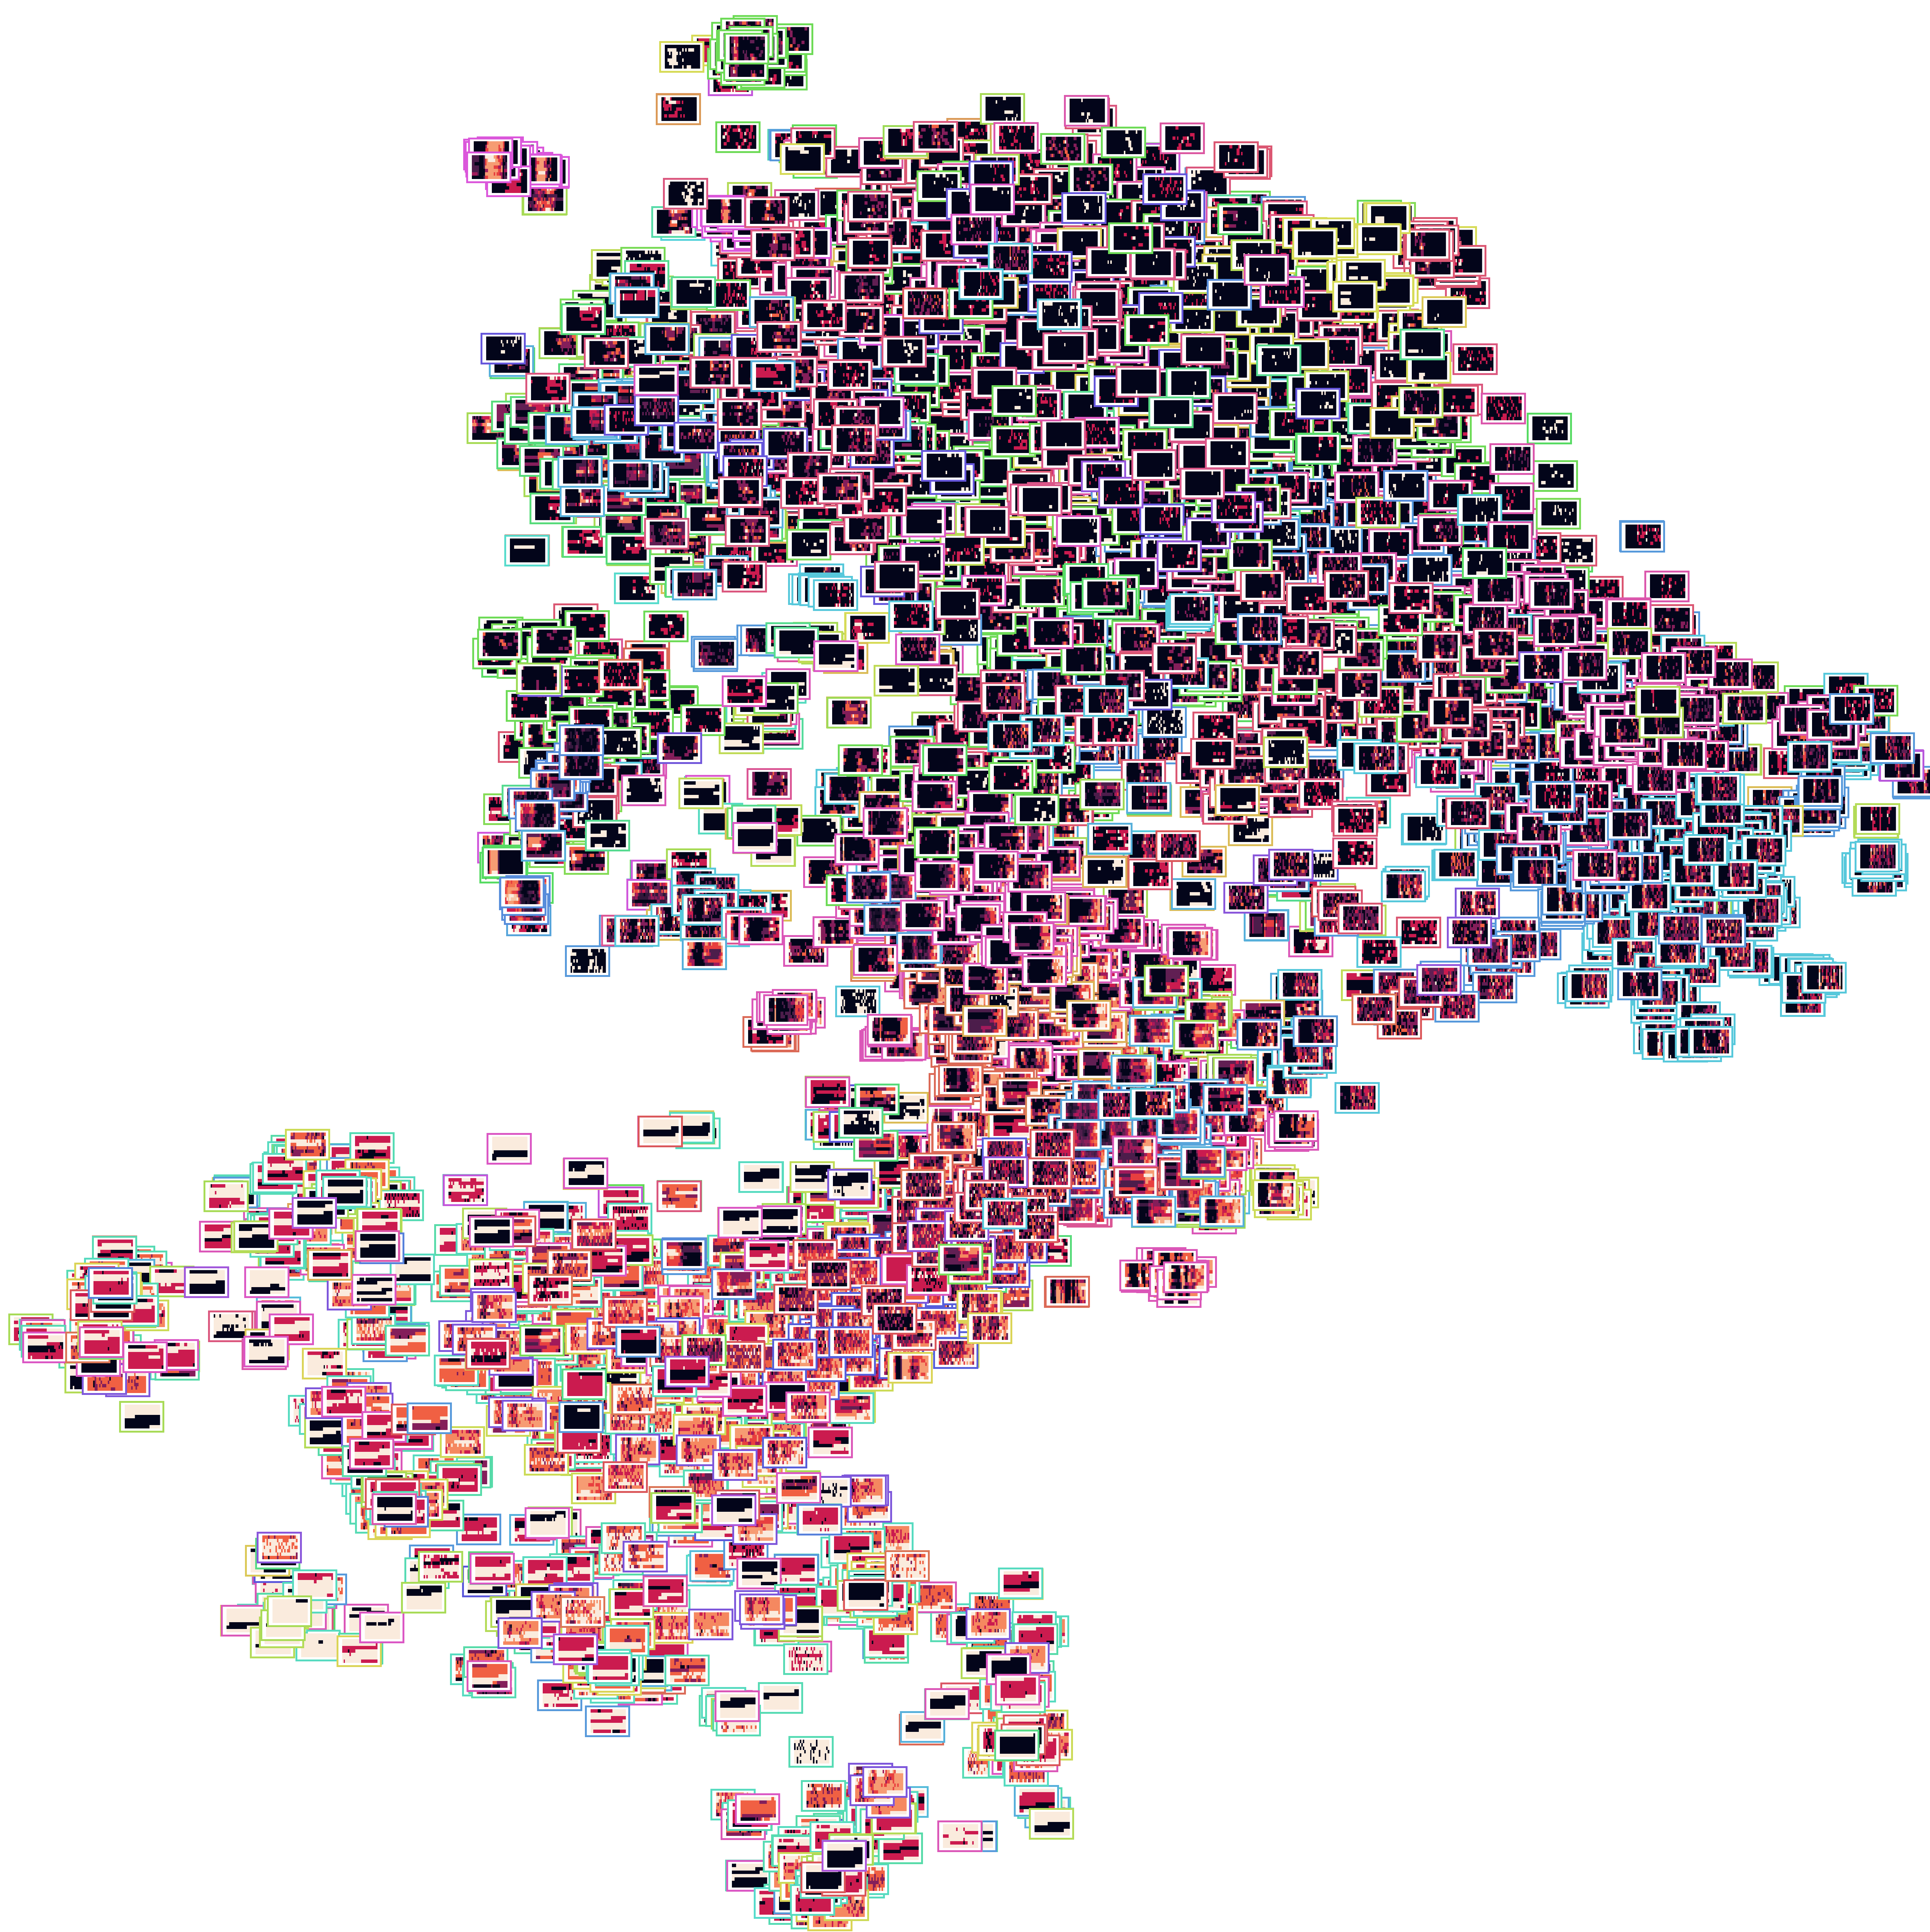
\includegraphics[width=.9\textwidth]{Figures/TSNE/TSNE_results/all/img_scatter_allall_lgimgs.png}
% 	\label{fig:tsne_papb_img_scatter_all}
% \end{figure}

To get a general idea of where each appliance group lies,
let's filter out all appliances that have less than 150 samples.
Applying this filter yields Figure \ref{fig:tsne_papb_scatter_all_reduced}.

\begin{figure}[H]
	\centering
	\caption{Projection of filtered per-appliance LPs}
	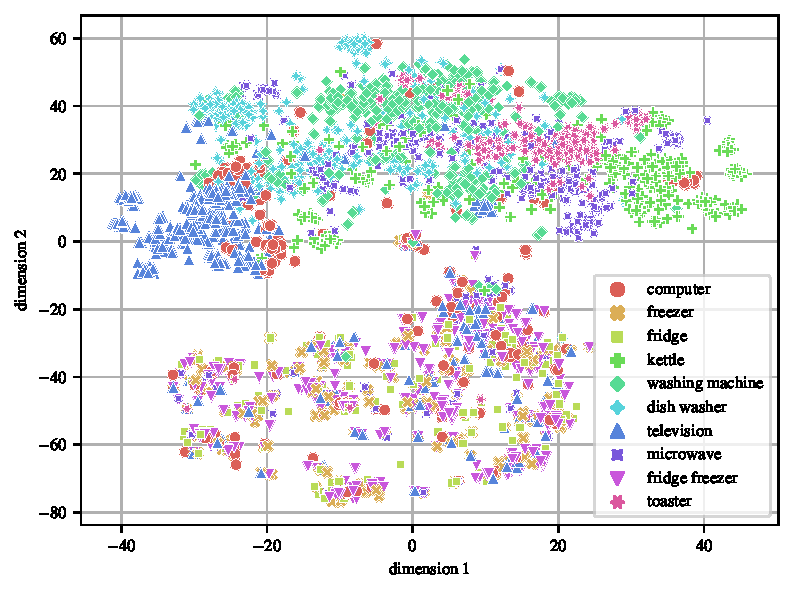
\includegraphics[]{Figures/TSNE/TSNE_PHPA/phpa_reduced_15.pdf}
	\label{fig:tsne_papb_scatter_all_reduced}
	\par
	\par\footnotesize{Full resolution figure: \url{https://github.com/jenkoj/msc/tree/main/Figures/TSNE/TSNE_PHPA/phpa_reduced_15.pdf}}
\end{figure}

Figure \ref{fig:tsne_papb_scatter_all_reduced} shows how these 10 appliances are connected in high dimensional space.
Kettles, microwaves and toasters are quite similar when it comes to usage patterns.
They are operated for a short amount of time and are usually used in users' routines in the morning or evening.
These appliances are located in the upper left part of the plot.

The second group of appliances that are quite near each other is white
goods (without fridges) such as washing machines, dishwashers, dryers etc.
Let's say that they are white goods with a program. 
This group of appliances is located in the upper right part of the plot.

The third group of appliances is white goods with a compressor.
They are usually not affected by human interaction and are therefore harder to cluster.
They are located in the lower part of the plot.

The final group of appliances is televisions and computers. They lie 
on a bridge between the fridges and other groups. 

% \begin{figure}[H]
% 	\centering
% 	\caption{Projection of filtered per-appliance LPs with actual samples}
% 	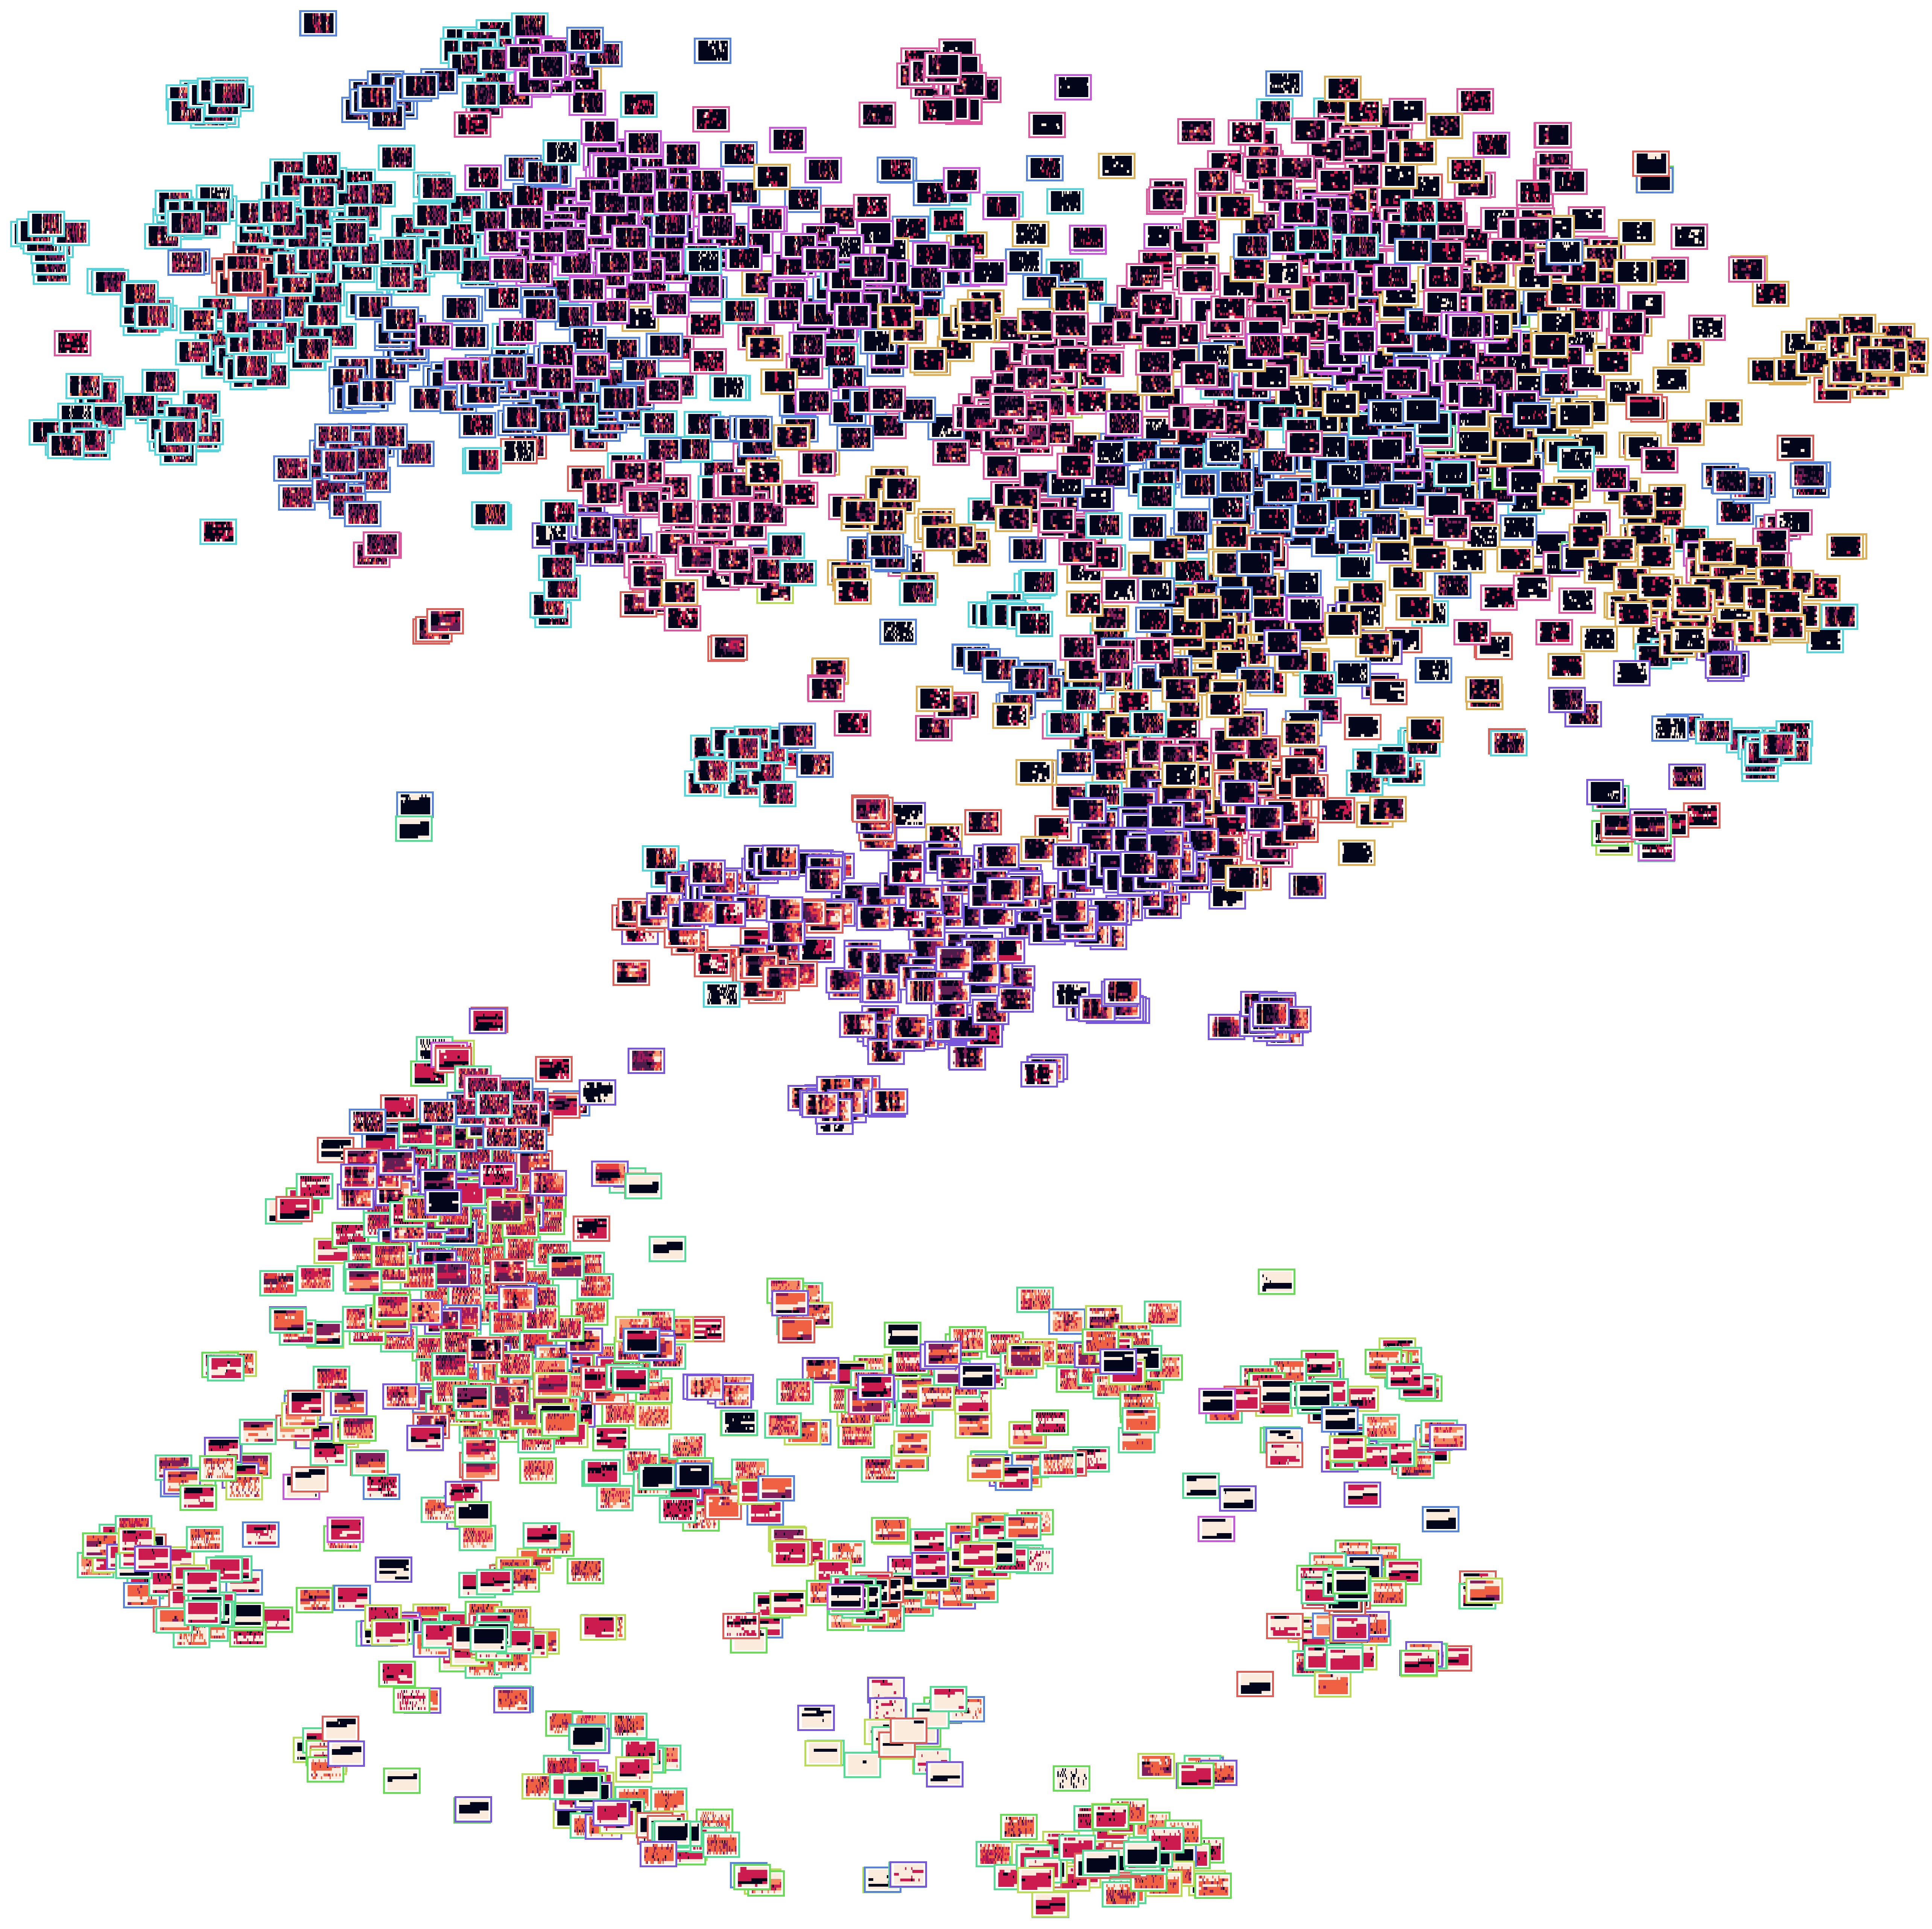
\includegraphics[width=.9\textwidth]{Figures/TSNE/TSNE_results/all/img_scatter_allall_reduced_max.png}
% 	\label{fig:tsne_papb_img_scatter_all_reduced}
% \end{figure}

% Even though the set of LPs is different due to filtering,
% the Figure \ref{fig:tsne_papb_img_scatter_all_reduced},
% retains a similar structure to the previous Figure \ref{fig:tsne_papb_scatter_all_reduced}. 

Knowing that a pattern exists, we can use the newly found group to define new appliance groups.
The following 8 groups will be defined
\begin{itemize}
    \item Kitchen appliances - toasters, ovens, microwaves, etc.
    \item Fridges and freezers  - contains fridges, freezers and fridge freezers or white goods with a compressor
    \item White goods - washers, dryers, dishwashers i.e. white goods with a program
    \item heating and cooling - Electric radiators, dehumidifiers and HVACs
    \item leisure -  Living room appliances such as TVs, games consoles, audio amps, HTPCs, etc.
    \item home office - Computer, laptops, printers, network equipment, chargers, etc.
    \item lightning - lights and lamps
    \item Others - unknown and unlabeled appliances
\end{itemize}

Applying these groups yields Figure \ref{fig:tsne_papb_scatter_all_groups}.
The new plot shows how, although appliances could be used by a different
user, maybe even by users in a different part of the EU or world,
they can be grouped in a high-dimensional space. 

\begin{figure}[H]
	\centering
	\caption{Projection of grouped per-appliance LPs}
	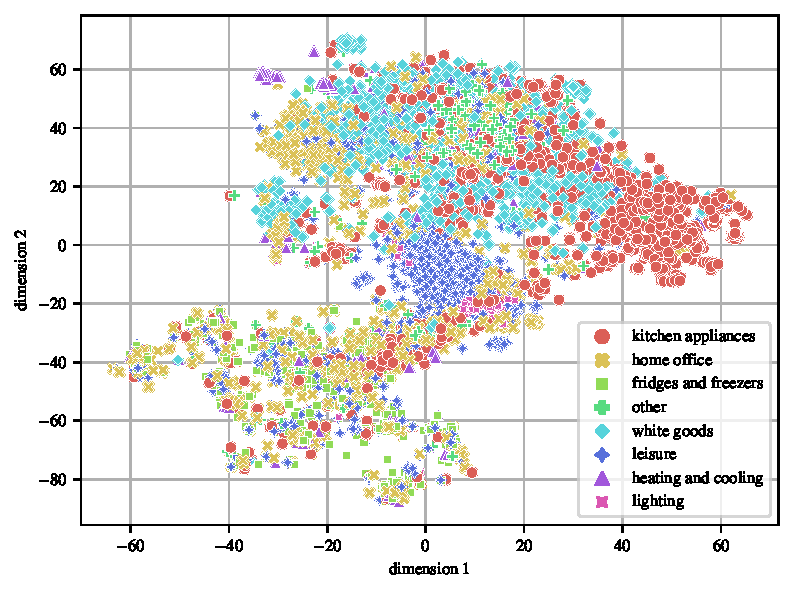
\includegraphics[]{Figures/TSNE/TSNE_PHPA/phpa_grouped_15.pdf}
	\label{fig:tsne_papb_scatter_all_groups}
	\par
	\par\footnotesize{Full resolution figure: \url{https://github.com/jenkoj/msc/tree/main/Figures/TSNE/TSNE_PHPA/phpa_grouped_15.pdf}}
\end{figure} 

The Figure \ref{fig:tsne_papb_img_scatter_all_groups} below is the same as the first Figure \ref{fig:tsne_papb_img_scatter_all} in the subsection,
except it is easier to use color to see the appliance they present

\begin{figure}[H]  
	\centering
	\caption{Projection of grouped per-appliance LPs with actual samples}
	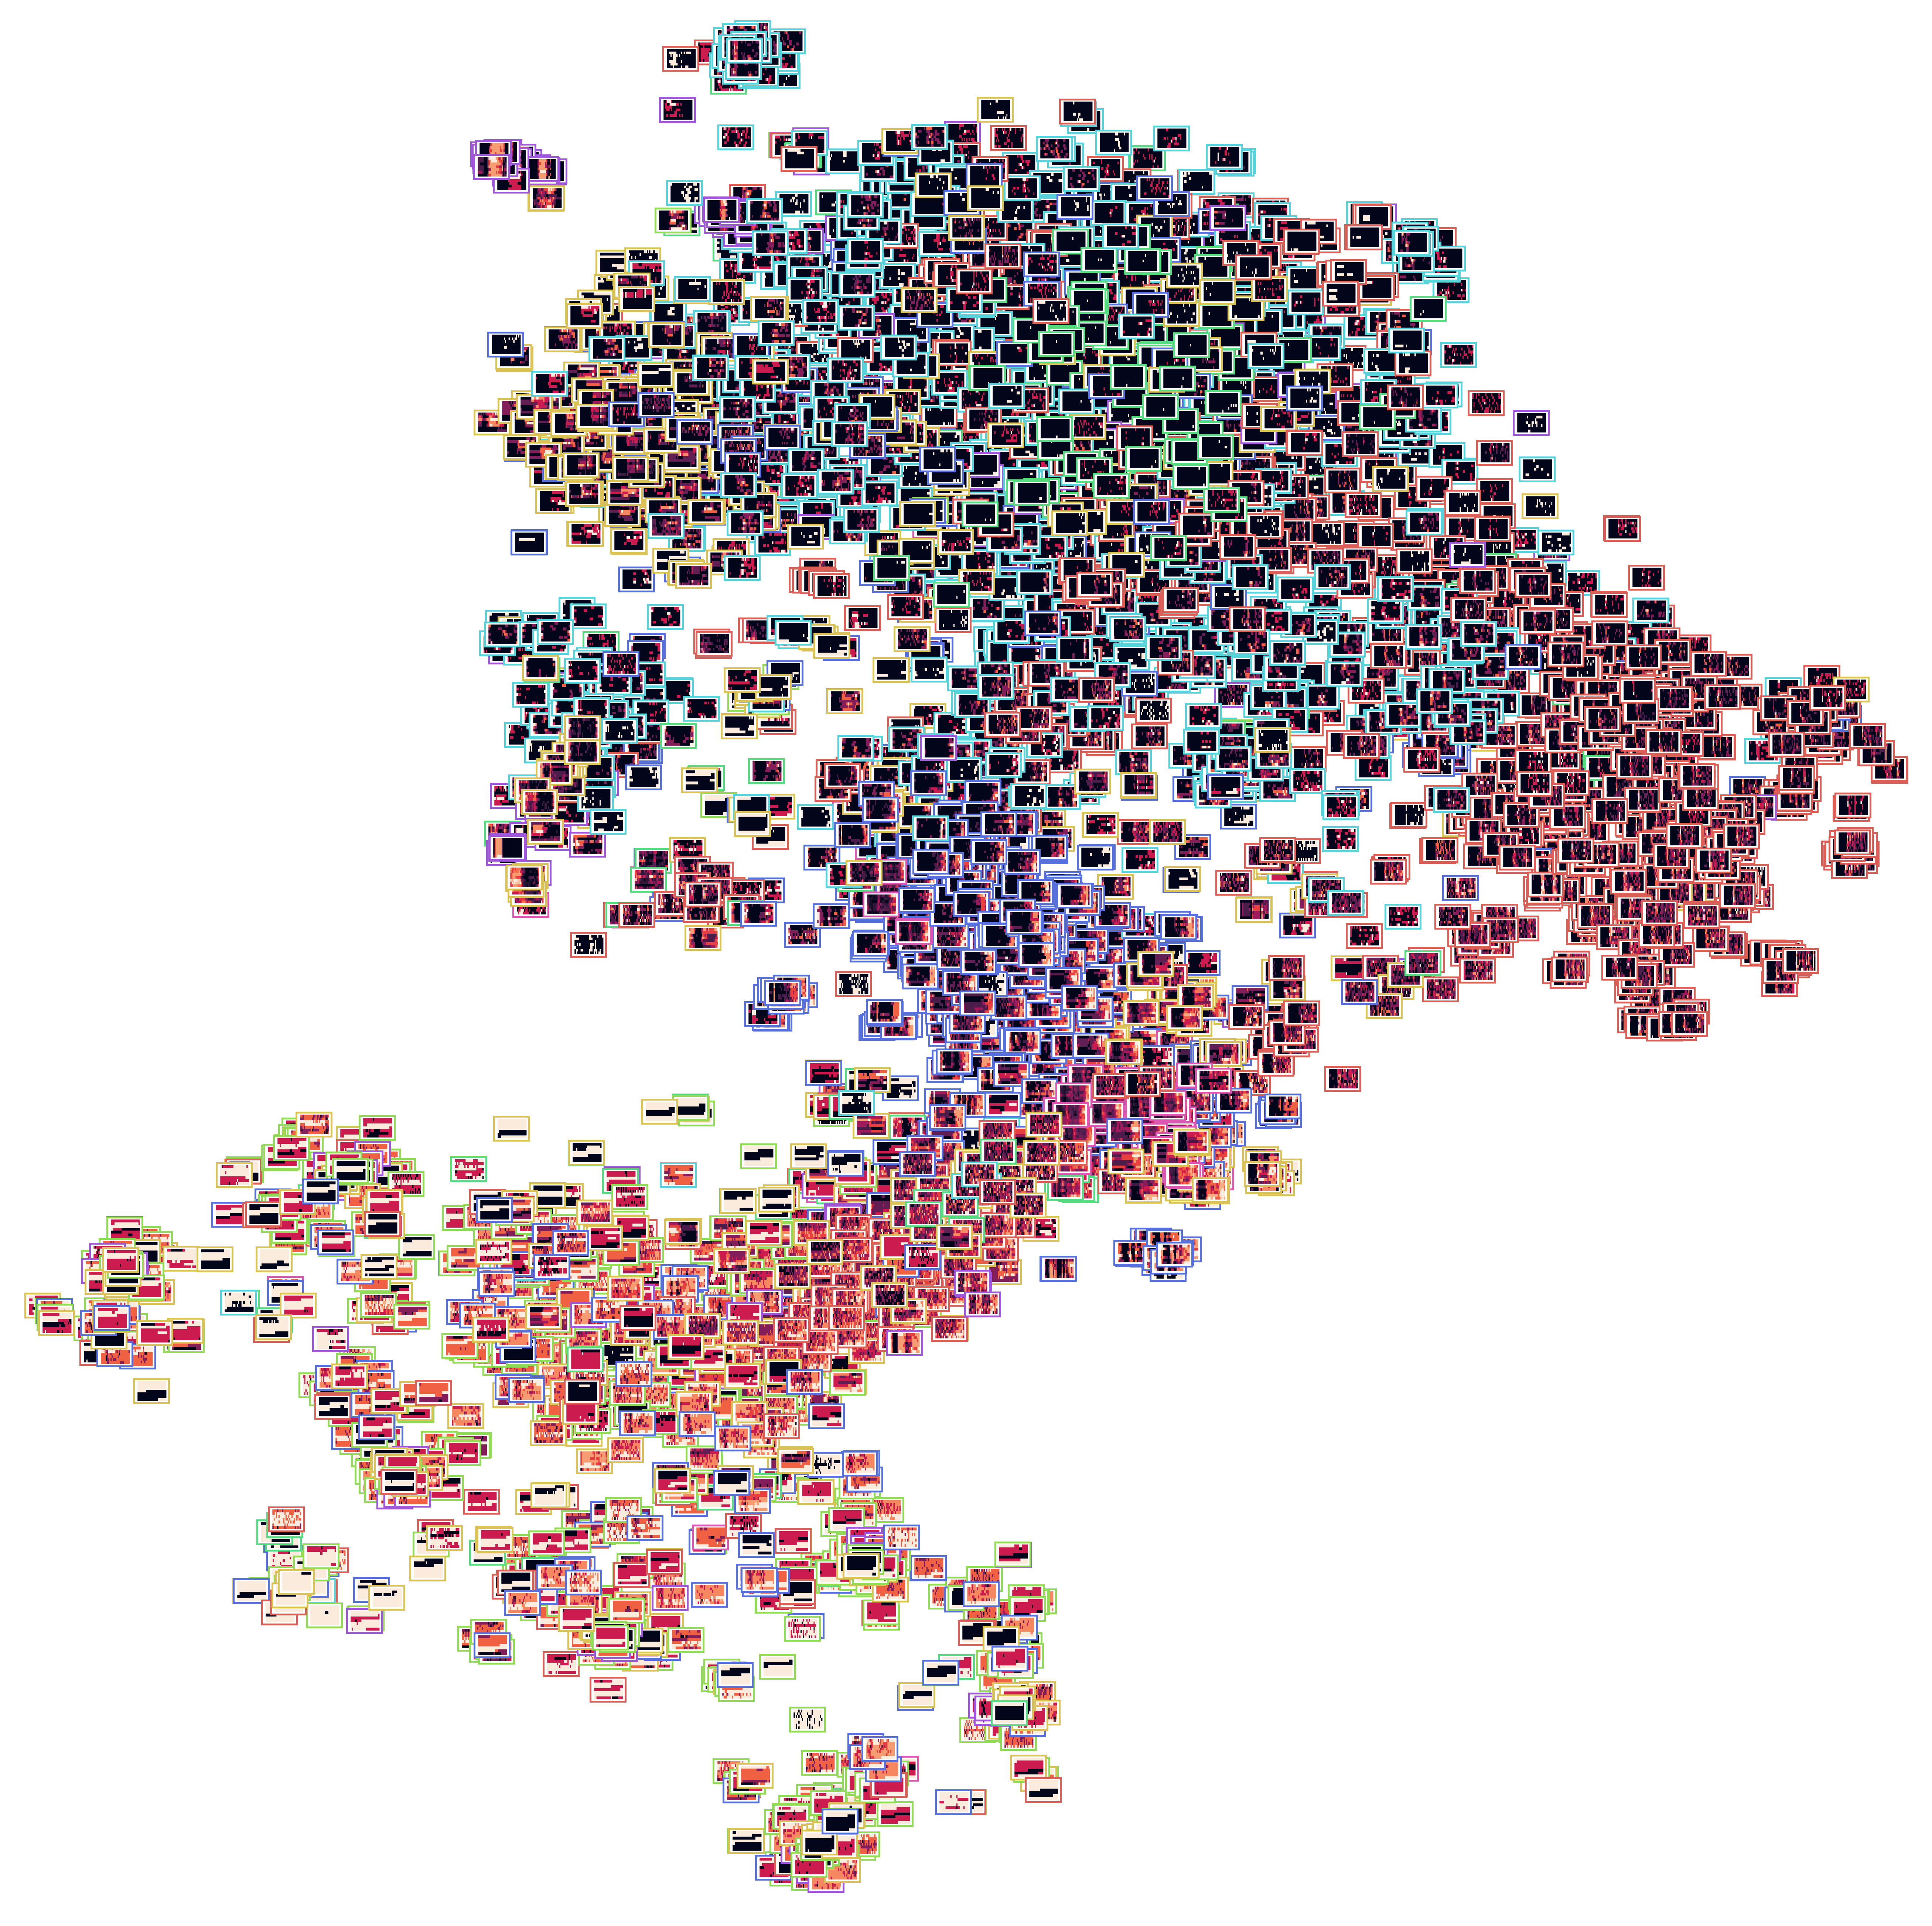
\includegraphics[width=1.1\textwidth]{Figures/TSNE/TSNE_PHPA/img_scatter_all_all_groups.png}
	\label{fig:tsne_papb_img_scatter_all_groups}
	\par
	\par\footnotesize{Full resolution figure: \url{https://github.com/jenkoj/msc/tree/main/Figures/TSNE/TSNE_PHPA/img_scatter_all_all_groups.png}}
\end{figure}

To better emphasize the details from Figure \ref{fig:tsne_papb_img_scatter_all_groups} and \ref{fig:tsne_papb_scatter_all_groups} we present zoomed-in areas of key locations with Figure \ref{fig:t-sne_zoomed}.
\begin{figure}[H] 
	\centering
	\caption{Projection of grouped per-appliance LPs with actual samples}
	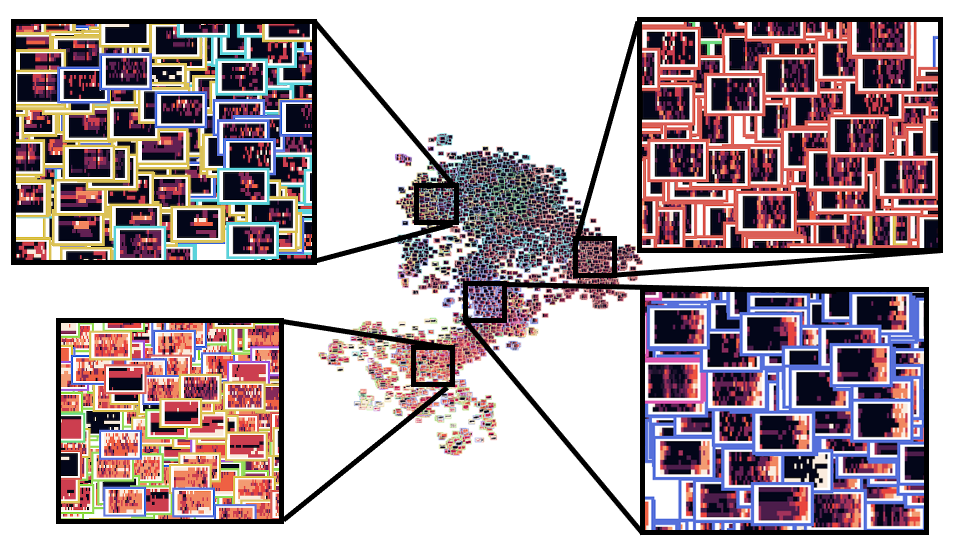
\includegraphics[width=1\textwidth]{Figures/TSNE/TSNE_PHPA/t-sne_zoomed.png}
	\label{fig:t-sne_zoomed}
	\par
	\par\footnotesize{Full resolution figure: \url{https://github.com/jenkoj/msc/tree/main/Figures/TSNE/TSNE_PHPA/t-sne_zoomed.png}}
\end{figure}

% One issue that causes the t-SNE algorithm an issue is low entropy data or 
% in other words, images that are almost completely dark or white, due to various faults in appliances or measurements.

% If we calculate the entropy for each image and set a threshold, it is possible to filter out these samples. 
% By setting an entropy threshold of 0.5, we filter out around 5 \% of all samples. 

% \begin{figure}[H]
% 	\centering
% 	\caption{Projection of entropy filtered per-appliance LPs}
% 	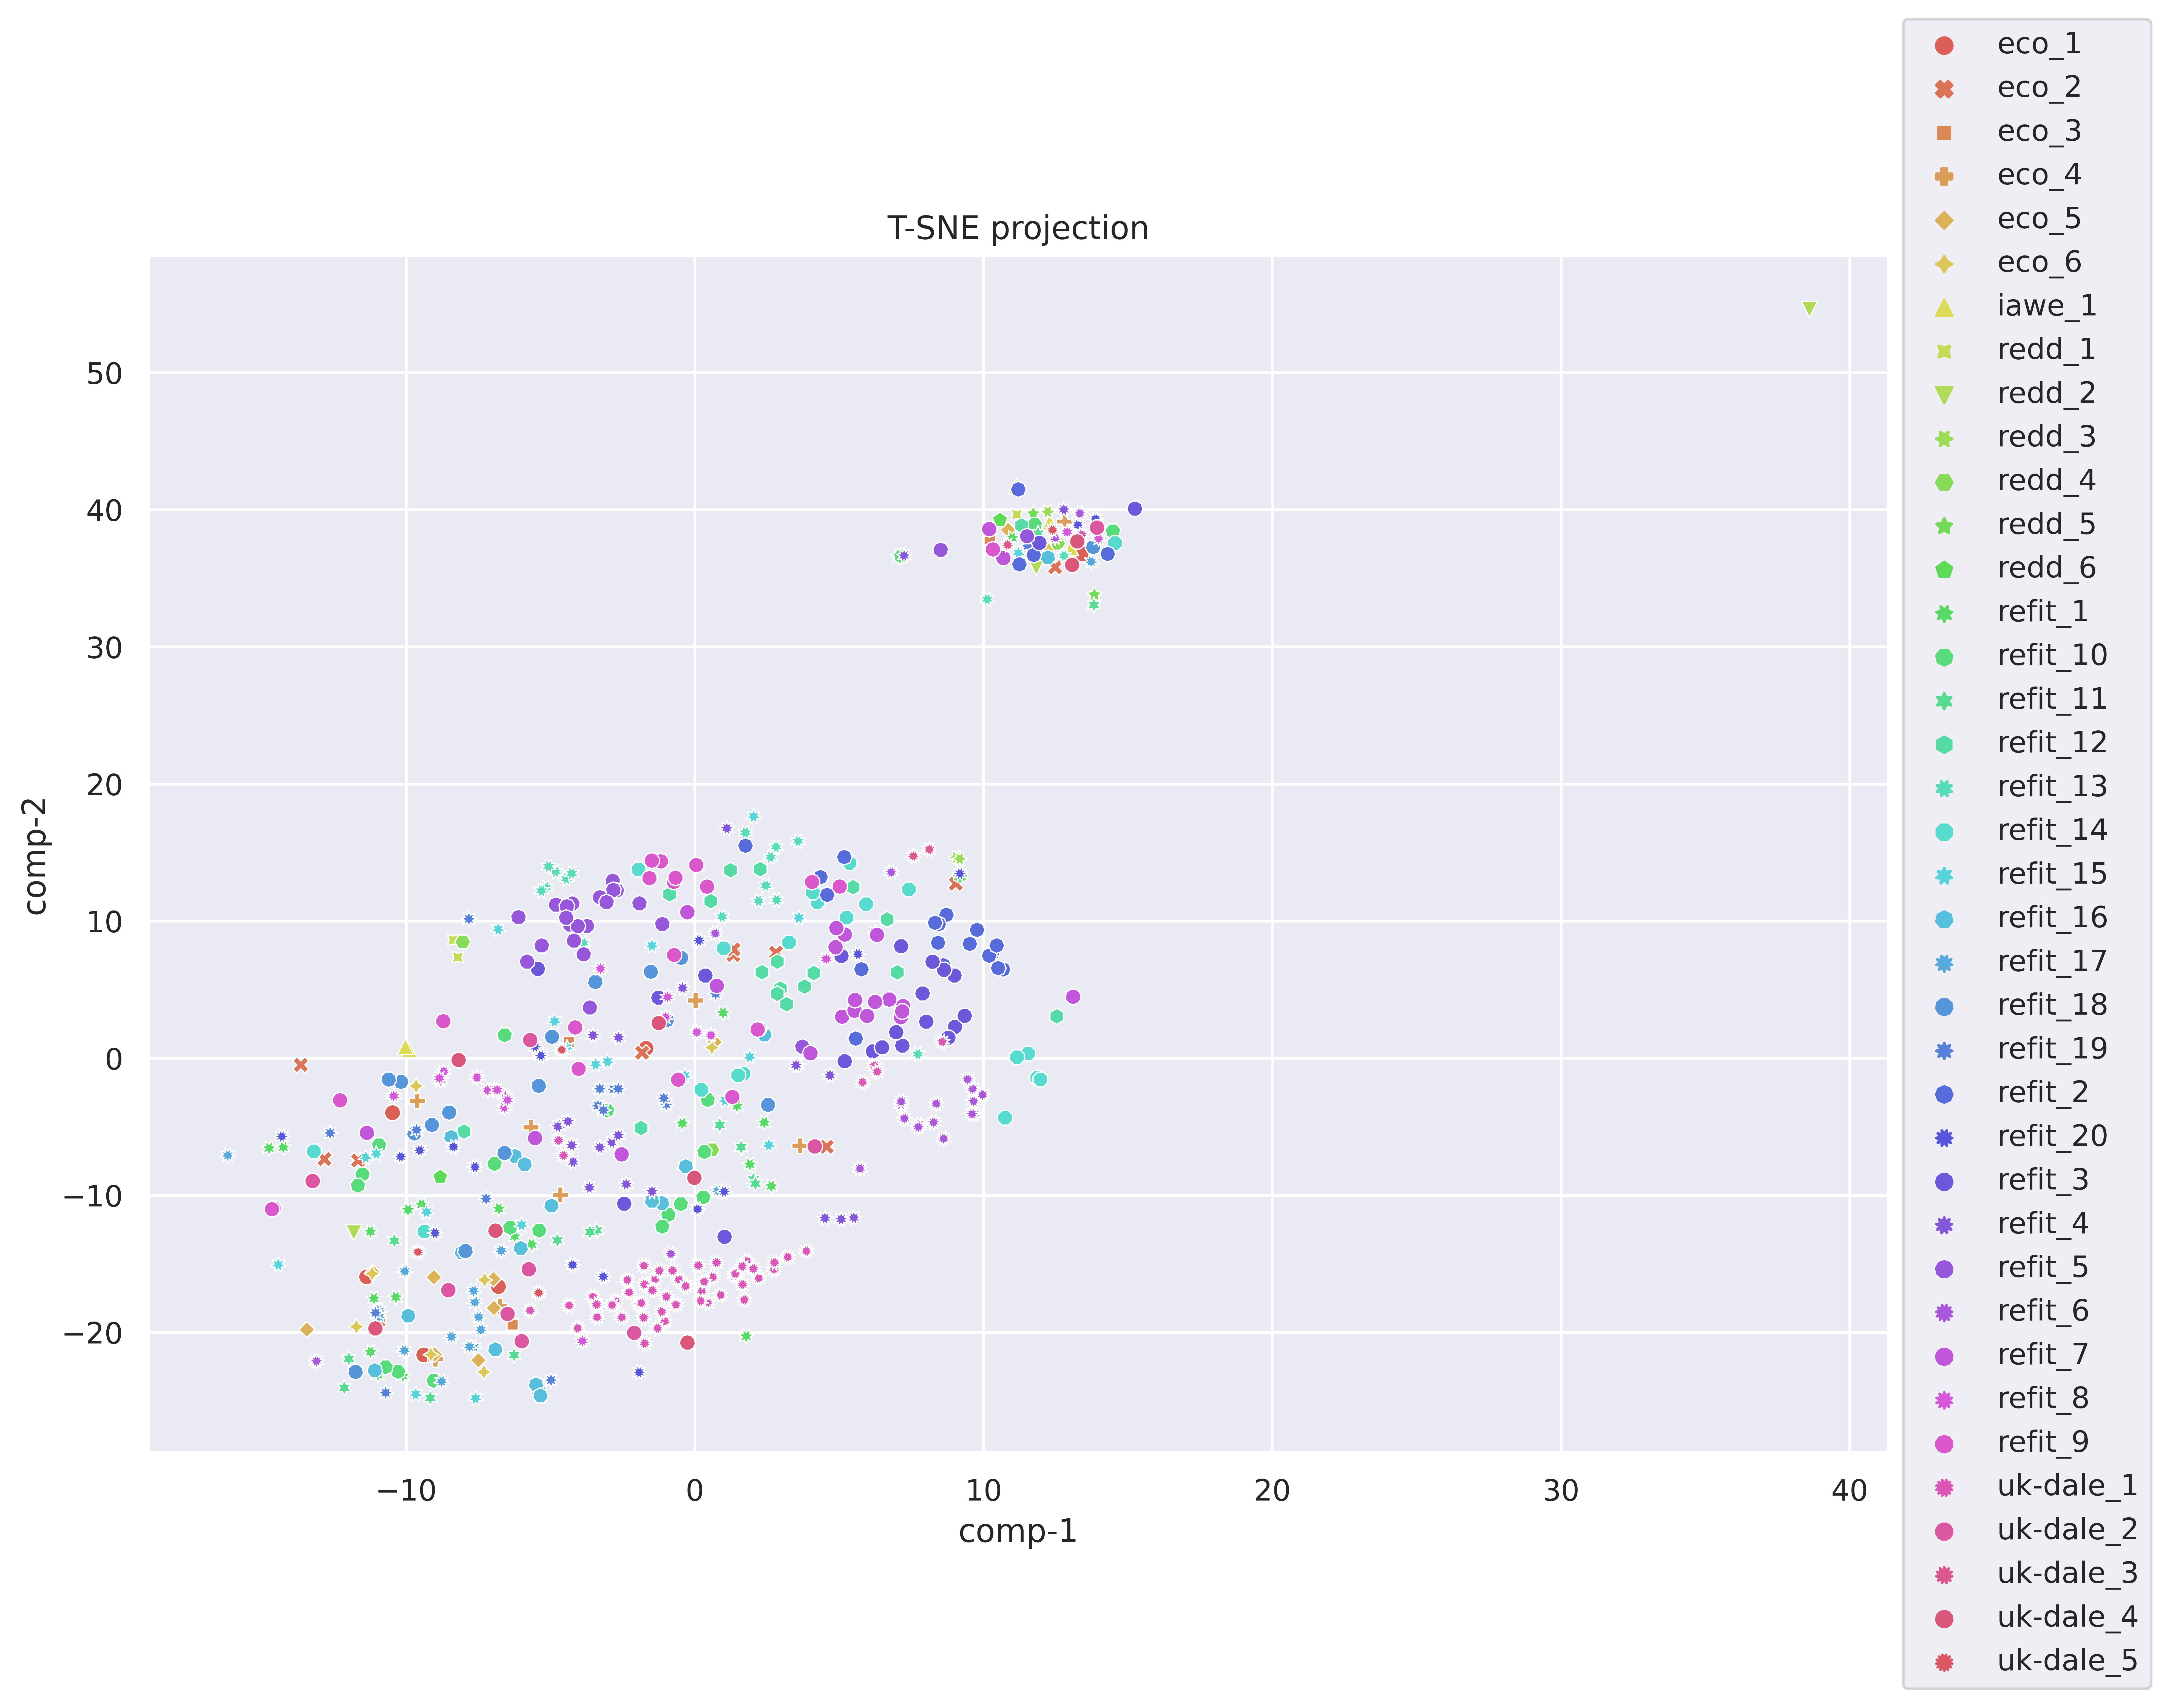
\includegraphics[width=.8\textwidth]{Figures/TSNE/TSNE_results_entropy/all/scatter_all_all.png}
% 	\label{fig:tsne_papb_scatter_ent_all_groups}
% \end{figure}

% Again, we can apply appliance grouping and get nicely formed clusters, such as can be seen in Figure \ref{fig:tsne_papb_img_scatter_ent_all_groups}.

% \begin{figure}[H]
% 	\centering
% 	\caption{Projection of entropy filtered per-appliance LPs with actual samples}
% 	\includegraphics[width=.8\textwidth]{Figures/TSNE/TSNE_results_entropy/all/scatter_all_all_groups.png}
% 	\label{fig:tsne_papb_img_scatter_ent_all_groups}
% \end{figure}


% \subsubsection{Comparing Appliances in a Building}

% It is also possible to use per-appliance data to study
% individual buildings, and how each appliance is used.
% In this case, we have used building 8 from REFIT as an example.

% \begin{figure}[H]
% 	\centering
% 	\caption{Projection of per-appliance LPs in a single building}
% 	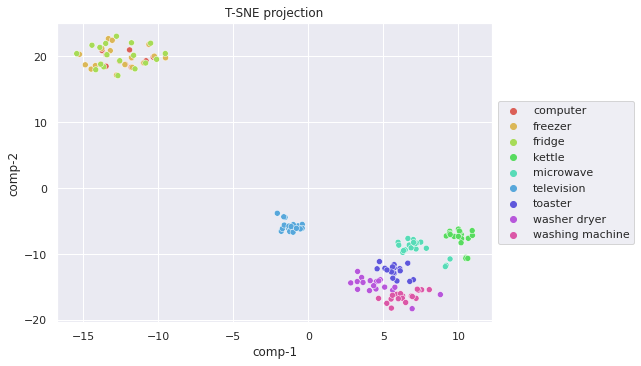
\includegraphics[width=.8\textwidth]{Figures/TSNE/TSNE_results/refit/scatter_refit_8.png}
% 	\label{fig:tsne_papb_scatter_ent_refit8}
% \end{figure}

% In general, the scattering is similar to before.
% Fridges and freezers are located opposite of white goods and kitchen appliances. 
% The television lies somewhere in between. 

% \begin{figure}[H]
% 	\centering
% 	\caption{Projection of per-appliance LPs in a single building with actual samples}
% 	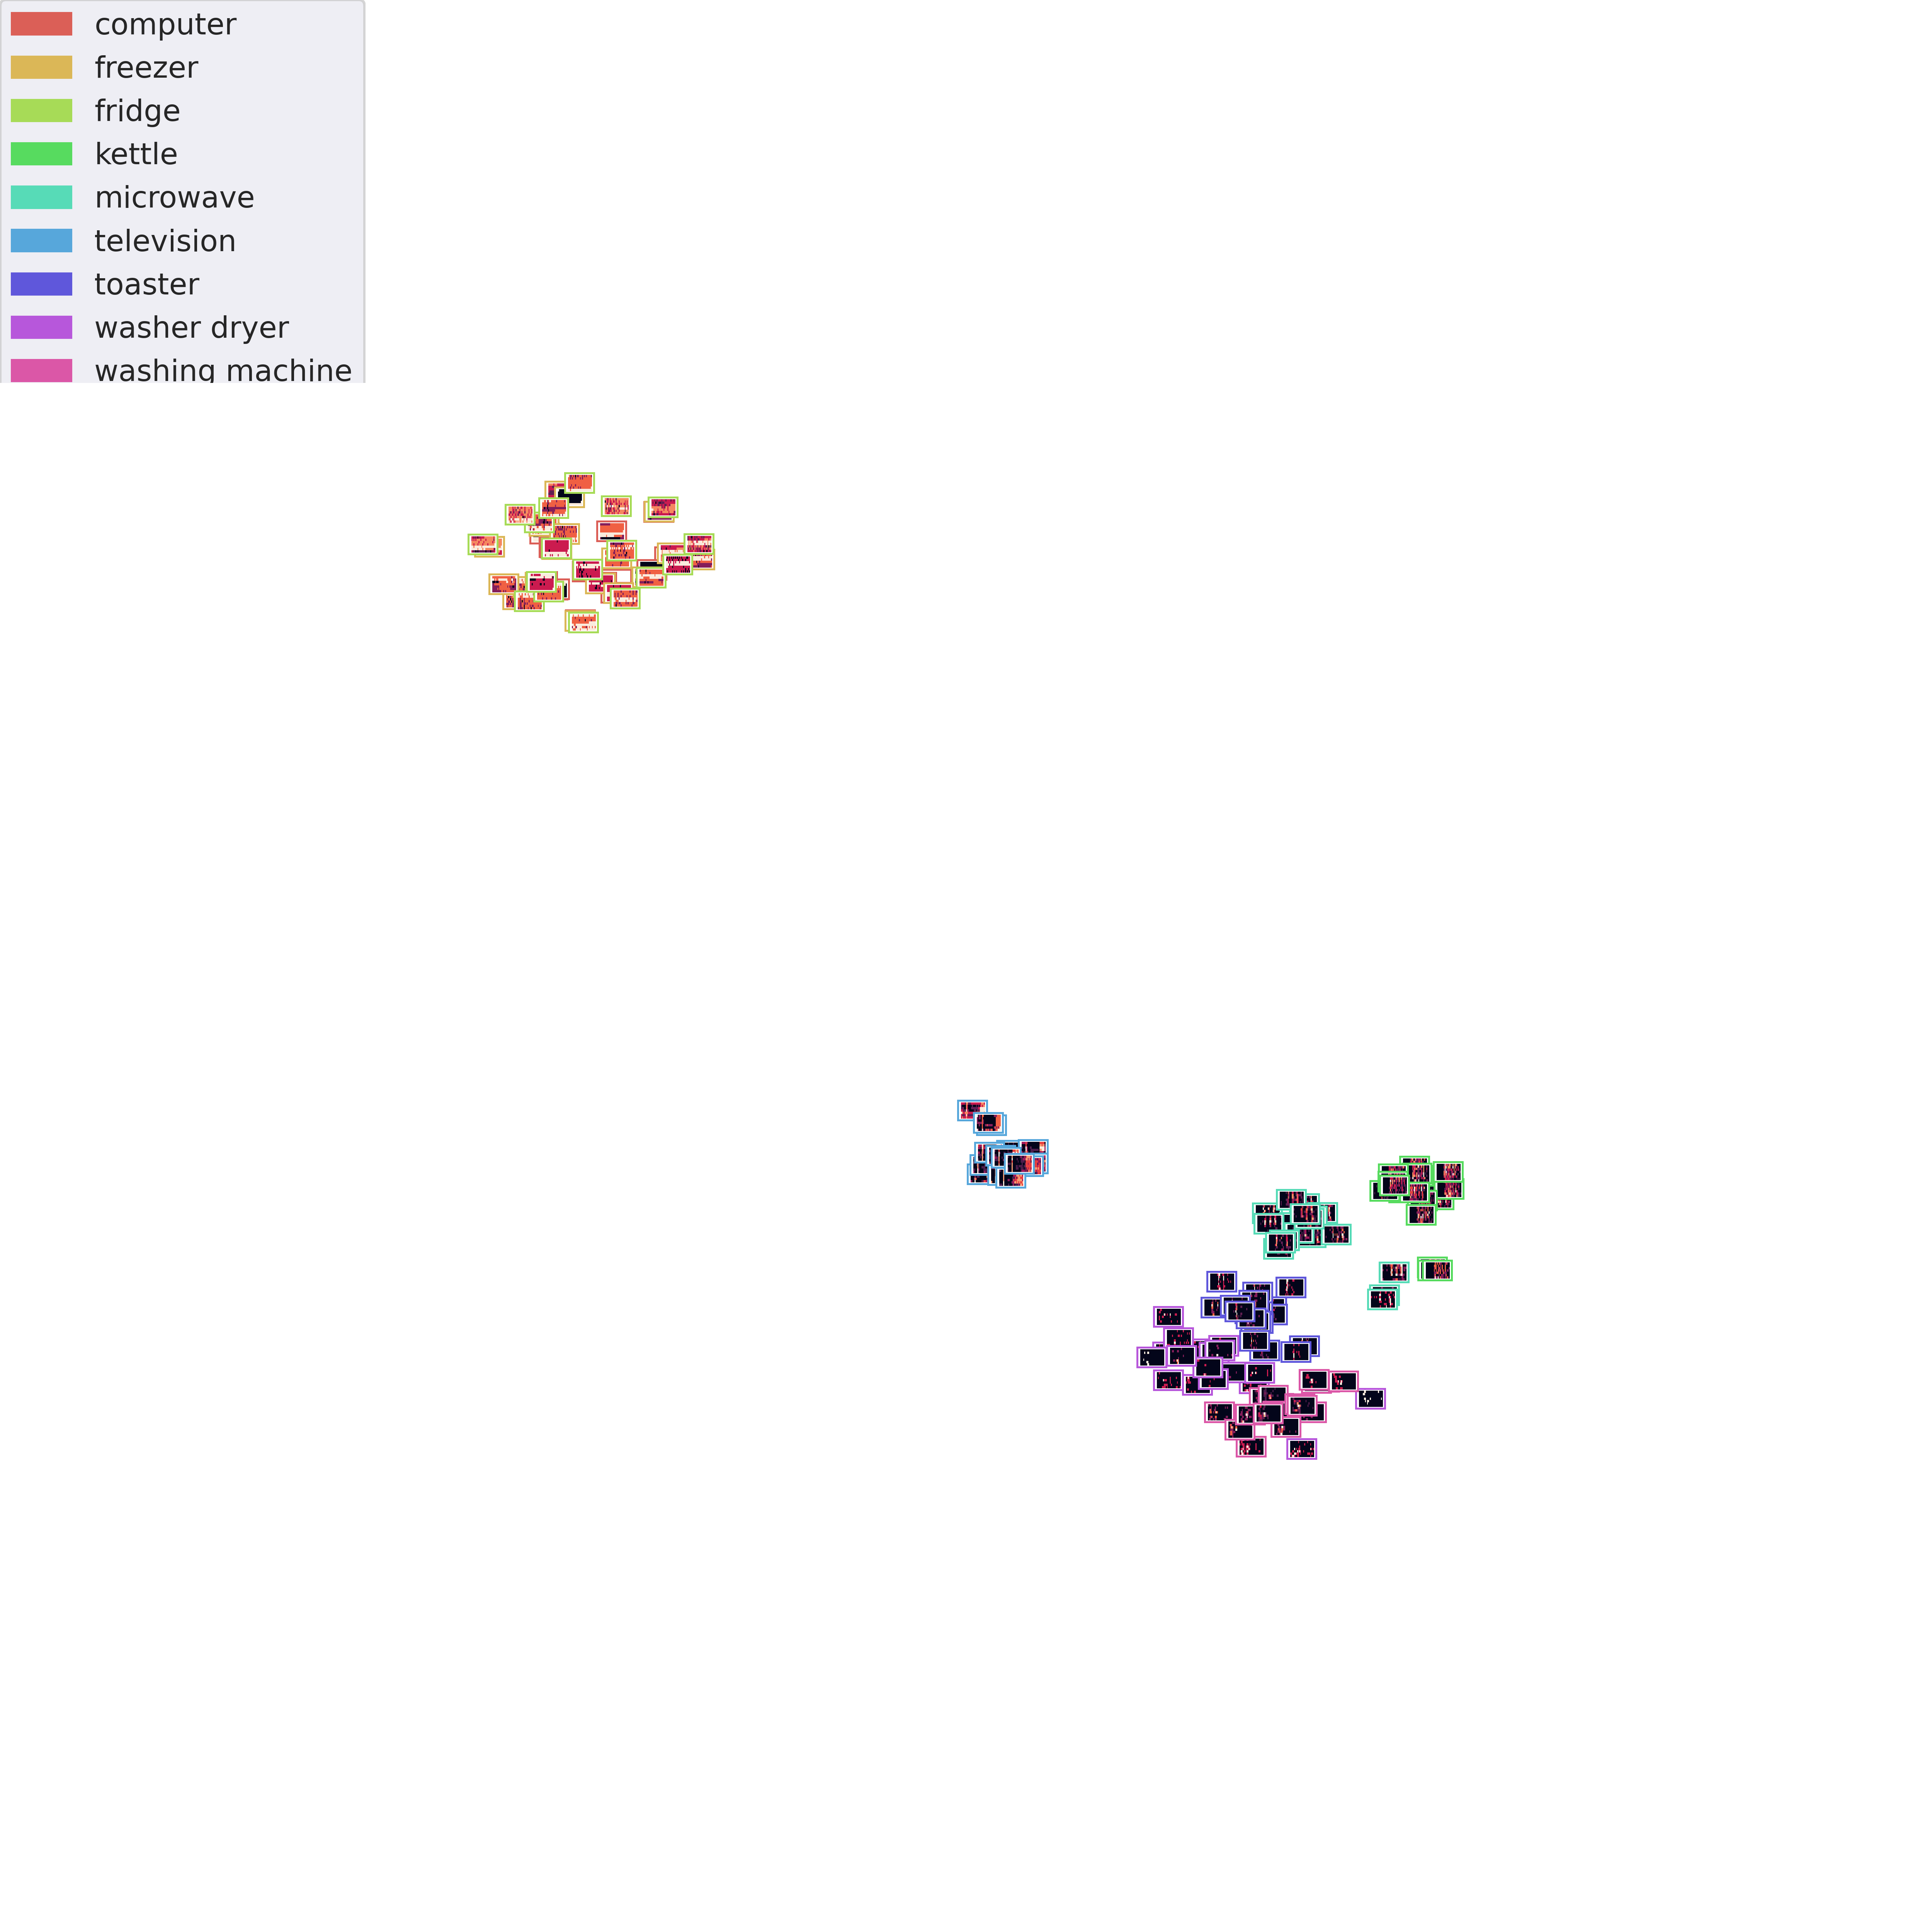
\includegraphics[width=.9\textwidth]{Figures/TSNE/TSNE_results/refit/img_scatter_refit8.png}
% 	\label{fig:tsne_papb_img_scatter_ent_refit8}
% \end{figure}

% Similar to before Figure \ref{fig:tsne_papb_img_scatter_ent_refit8} shows the fridge cluster as the most active,
% with the least interesting information. In the middle, we can again observe the TV that is mostly being used
% in the evening hours. The samples also point to the possibility of a high-user routine in the early morning hours.
% The high routine is portrayed as a straight line on the figures. 

% In this case, when observing white goods in pink and purple boxes, it is possible to see that this user primarily uses them during the night hours.
% This could point out that the user is making use of cheaper tariffs.

% One other interesting observation that can be made here is comparing kettles, microwaves and toasters.
% Usually, these appliances are used similarly and in similar parts of the day. 
% Here the toaster and microwave are being used periodically, but the kettle is being used throughout the day with no general pattern.
% It is self-obvious that some users have higher routines than others, but this observation
% would add that some users can have a higher routine for some appliances and lower for others, of the same type. 

\subsection{Per-Appliance Per-Building}

To study the usage by comparing all appliances between buildings,
we have to use one of the proposed LPs and in this case, this is a Bag of appliances.

\subsubsection{Bag of Appliances}

This LP is a combination of the LPs above,
except it offers a larger detail when observing groups of appliances.
Since we are using one dimension for appliances, we will use only the daily dimension.

To construct such a profile we need a universal way of constructing it.
This is done by measuring how many times each appliance occurs in the datasets,
then this list is sorted from most common to least common, and finally, the top 30 are selected.

The problem with such a comparison is, that it is best 
if all buildings would use the same appliances.
Since that is not the case, missing appliances are portrayed as always off. 

This is the main reason why we can see in Figure \ref{fig:tsne_boa_scatter_refit8} the clusters are separated quite a bit.
We can still see that some clusters are closer than others,
meaning they are more similar.  

\begin{figure}[H]
	\centering
	\caption{Projection of a bag of appliances LPs for various buildings}
	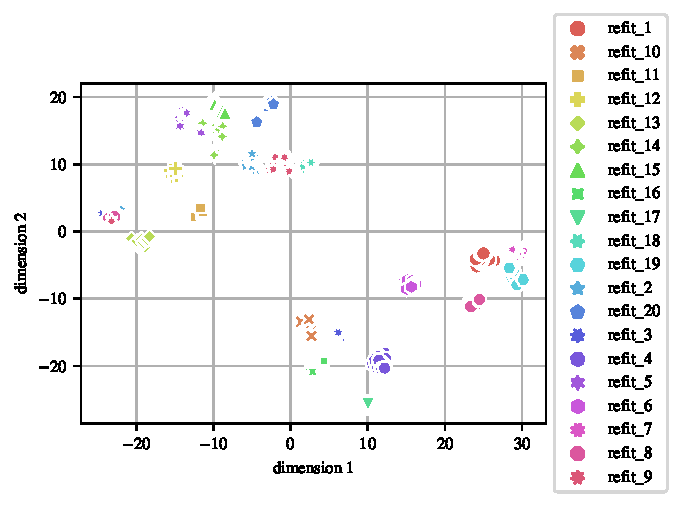
\includegraphics[]{Figures/TSNE/TSNE_BOA/scatter_refit_boa.pdf}
	\label{fig:tsne_boa_scatter_refit8}
	\par
	\par\footnotesize{Full resolution figure: \url{https://github.com/jenkoj/msc/tree/main/Figures/TSNE/TSNE_BOA/scatter_refit_boa.pdf}}
\end{figure} 

Figure \ref{fig:tsne_boa_img_scatter_refit8} shows that LPs are split 
between two poles. 
By observing the Figure it is possible to see that all the bottom clusters
have more than one active white good with a compressor (fridges and freezers), while
the top ones have only one. In general, the bottom buildings have more appliances,
with more activity than the top ones. 

\begin{figure}[H]
	\centering
	\caption{Projection of a bag of appliances LPs for various buildings with actual samples}
	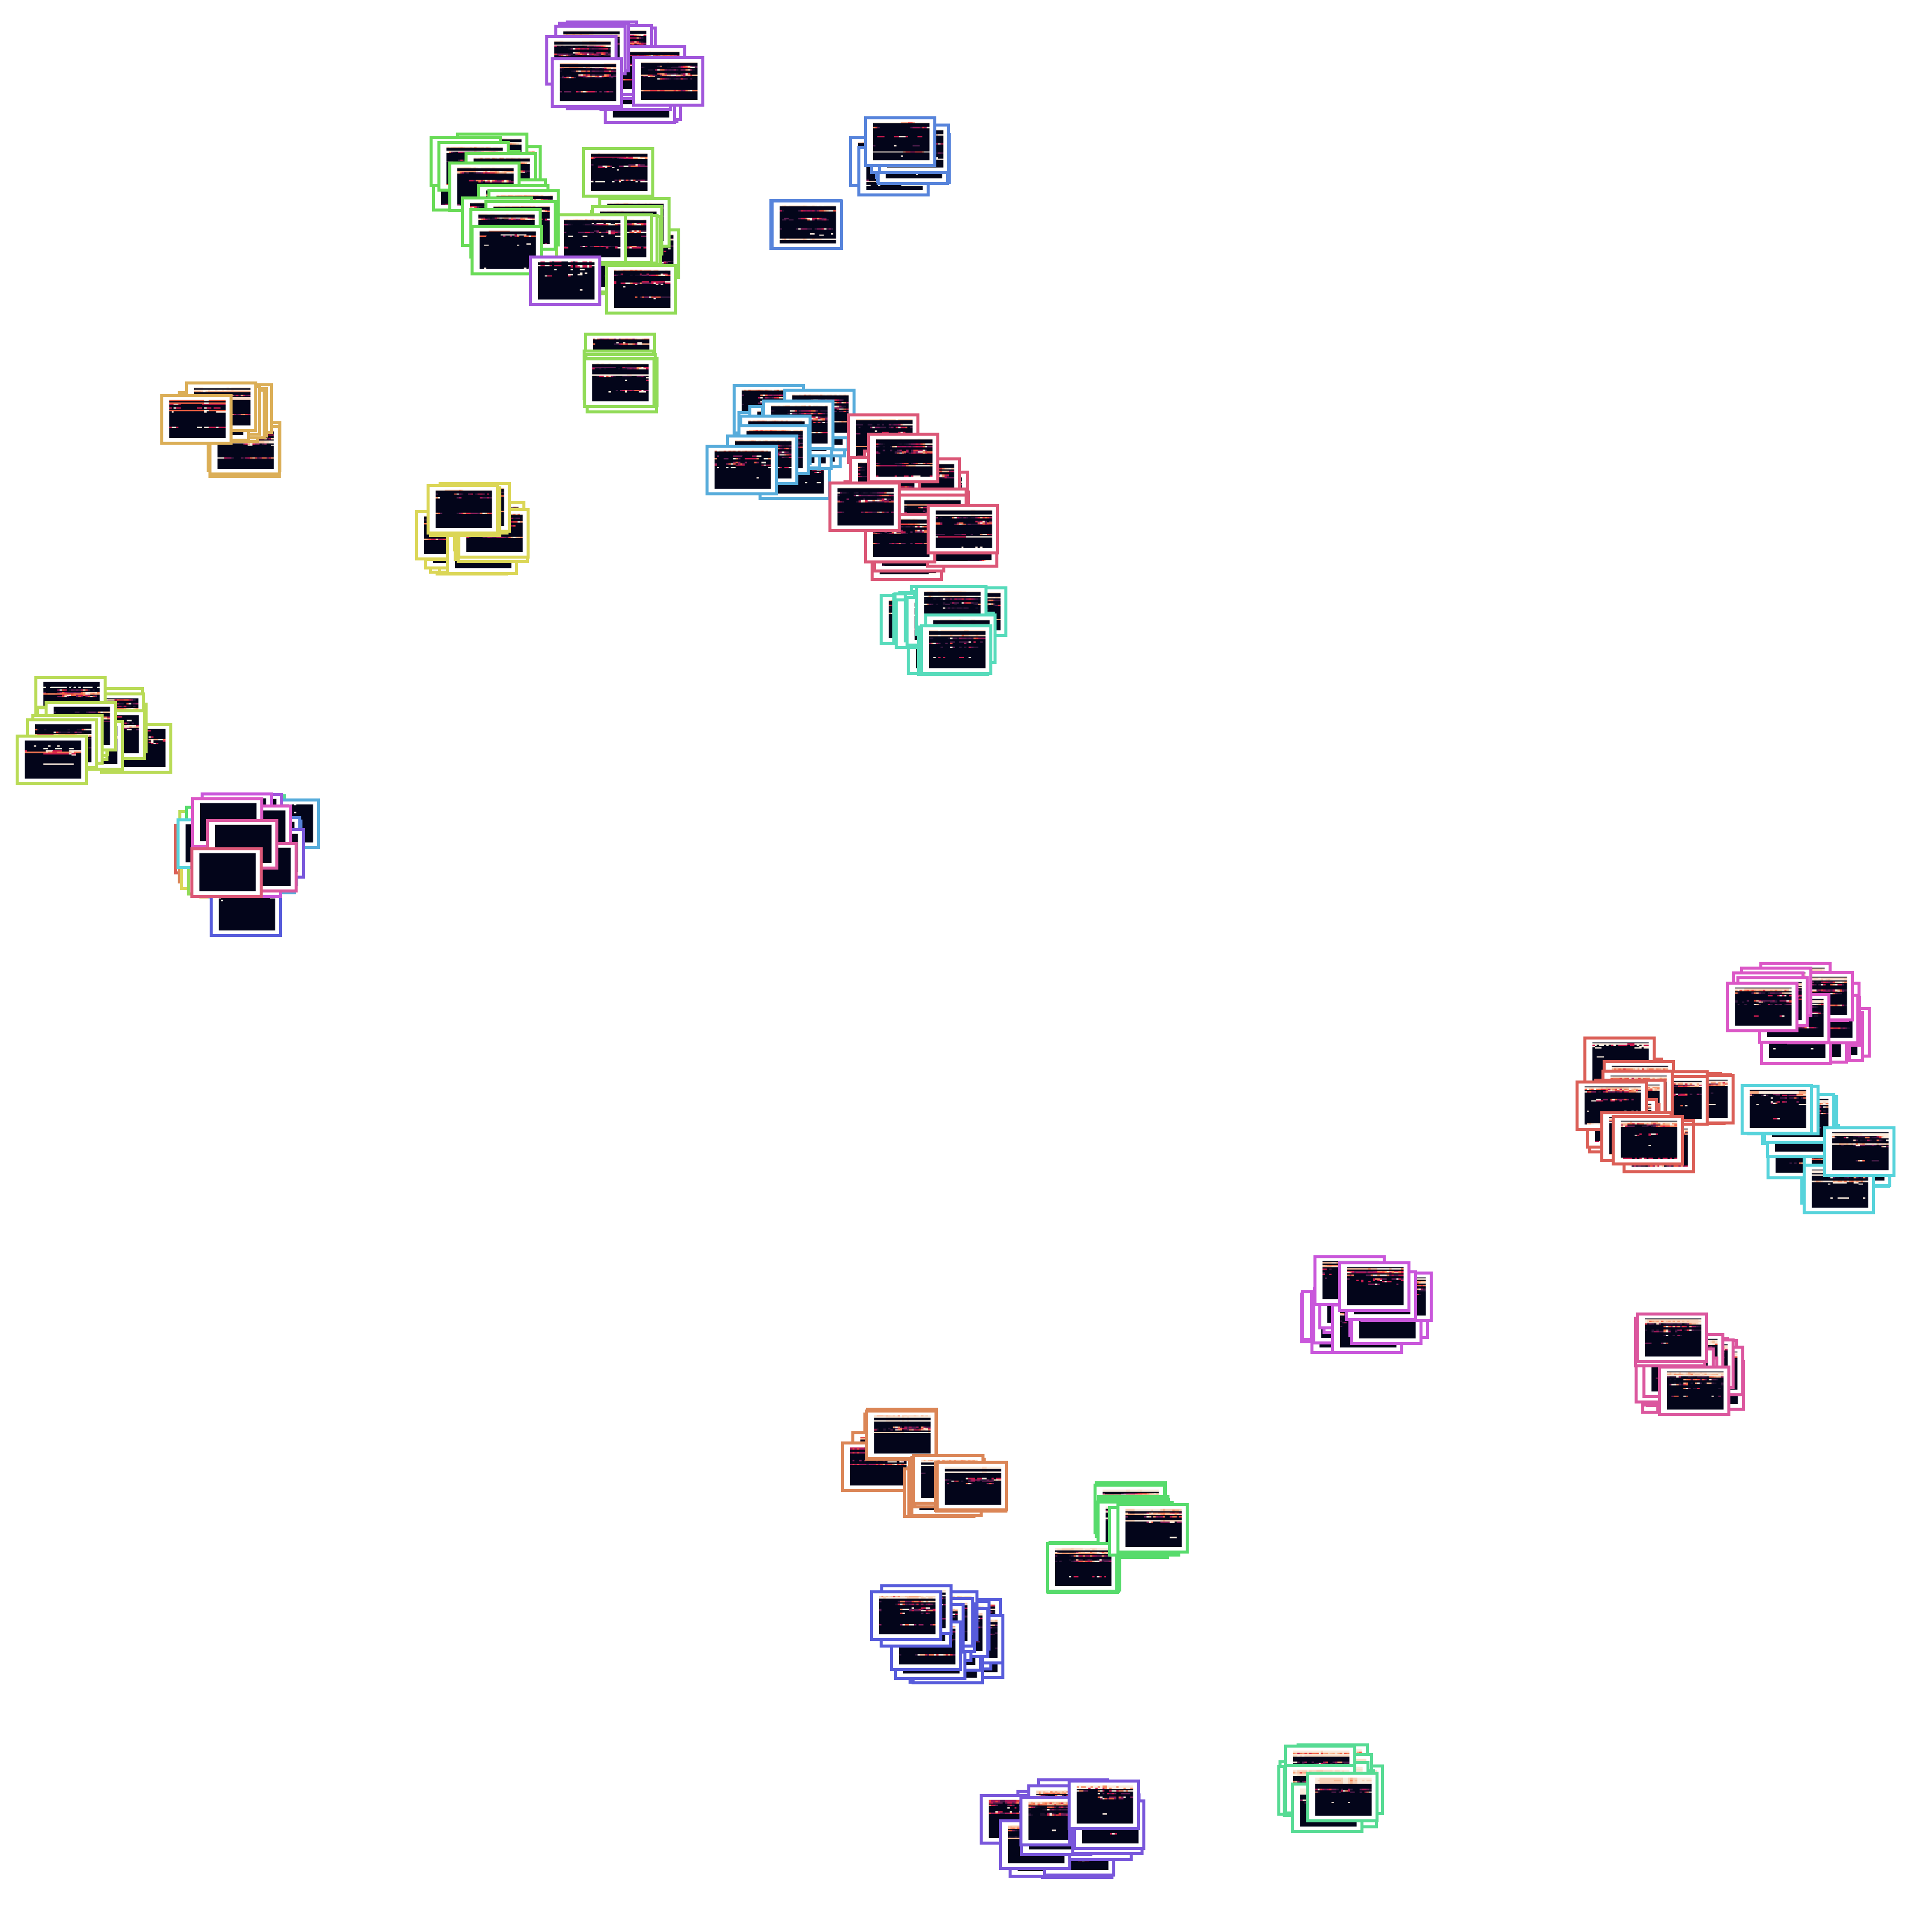
\includegraphics[width=.9\textwidth]{Figures/TSNE/TSNE_BOA/img_scatter_boa.png}
	\label{fig:tsne_boa_img_scatter_refit8}
	\par
	\par\footnotesize{Full resolution figure: \url{https://github.com/jenkoj/msc/tree/main/Figures/TSNE/TSNE_BOA/img_scatter_boa.png}}
\end{figure}

\section{Discussion}

We used t-SNE to show how LPs are related in high-dimensional space, by mapping them into two-dimensional space.
We used three different types of LPs: per-building, per-building per-appliance, a bag of appliances, and per-appliance.
Per-building load profiles offered a look into how activations patterns differ across different buildings and datasets.
Per-building per-appliance bag of appliance load profiles offered the same thing, but in greater detail.
Per-appliance load profiles were the most versatile and were utilized in the most various ways:
First, we have shown how the same type of appliance is being used across various buildings.
Next, we compared appliances with each other. 
Since the plot was hard to comprehend, we have defined appliance groups.
These new groups formed clusters, which furthermore revealed the relation between LPs. 
Finally, we compared how appliance load profiles are connected in a single building. 

One of the main findings of this chapter was the formation of appliance groups.
Such groups enable us to look into the similarity of their activation profiles and enable us to understand which groups have similar usage patterns.
Another important piece of information these groups contain is the strength of the user's routine.
The closer the samples, the more similar their activation is, which means the user has a higher routine.
Such a routine will be useful in the next chapter, where we will try to evaluate if it is strong enough to detect anomalies.

\section{Summary}

The analysis provided a look into the relationships between LPs and their consumption patterns.
We were able to group appliances into categories and found a presence of routine in the LPs
These findings will be valuable in the next chapter where we continue to explore the potential applications of LPs.

